
\subsubsection{Análisis para $C_{comp}$ en modo tensión, $V_{out} = 10 \si[per-mode=symbol]{\volt}$, $R_{L} = 10 \si[per-mode=symbol]{\ohm}$}

Se puede ver en la figura~\figref{fig:fig_power_supply_CCOMP_LOOP_Modo1} como ya con el valor de $C_{comp} = 10 \si[per-mode=symbol]{\nano\farad}$ se logra unos márgenes de fase y ganancia aceptables, seguir aumentando el valor de $C_{comp}$, solo disminuye innecesariamente el ancho de banda, como se puede ver en la figura~\figref{fig:fig_power_supply_CCOMP_RF_Modo1}. A nivel de respuesta dinámica no se ven grandes diferencias entre los valores simulados, ver figura~\figref{fig:fig_power_supply_CCOMP_STEP_5n_Modo1}, figura~\figref{fig:fig_power_supply_CCOMP_STEP_10n_Modo1} y figura~\figref{fig:fig_power_supply_CCOMP_STEP_20n_Modo1}.

\vfill


% CCOMP MODO 1.

\clearpage

\begin{figure}[H] %htb
\begin{center}
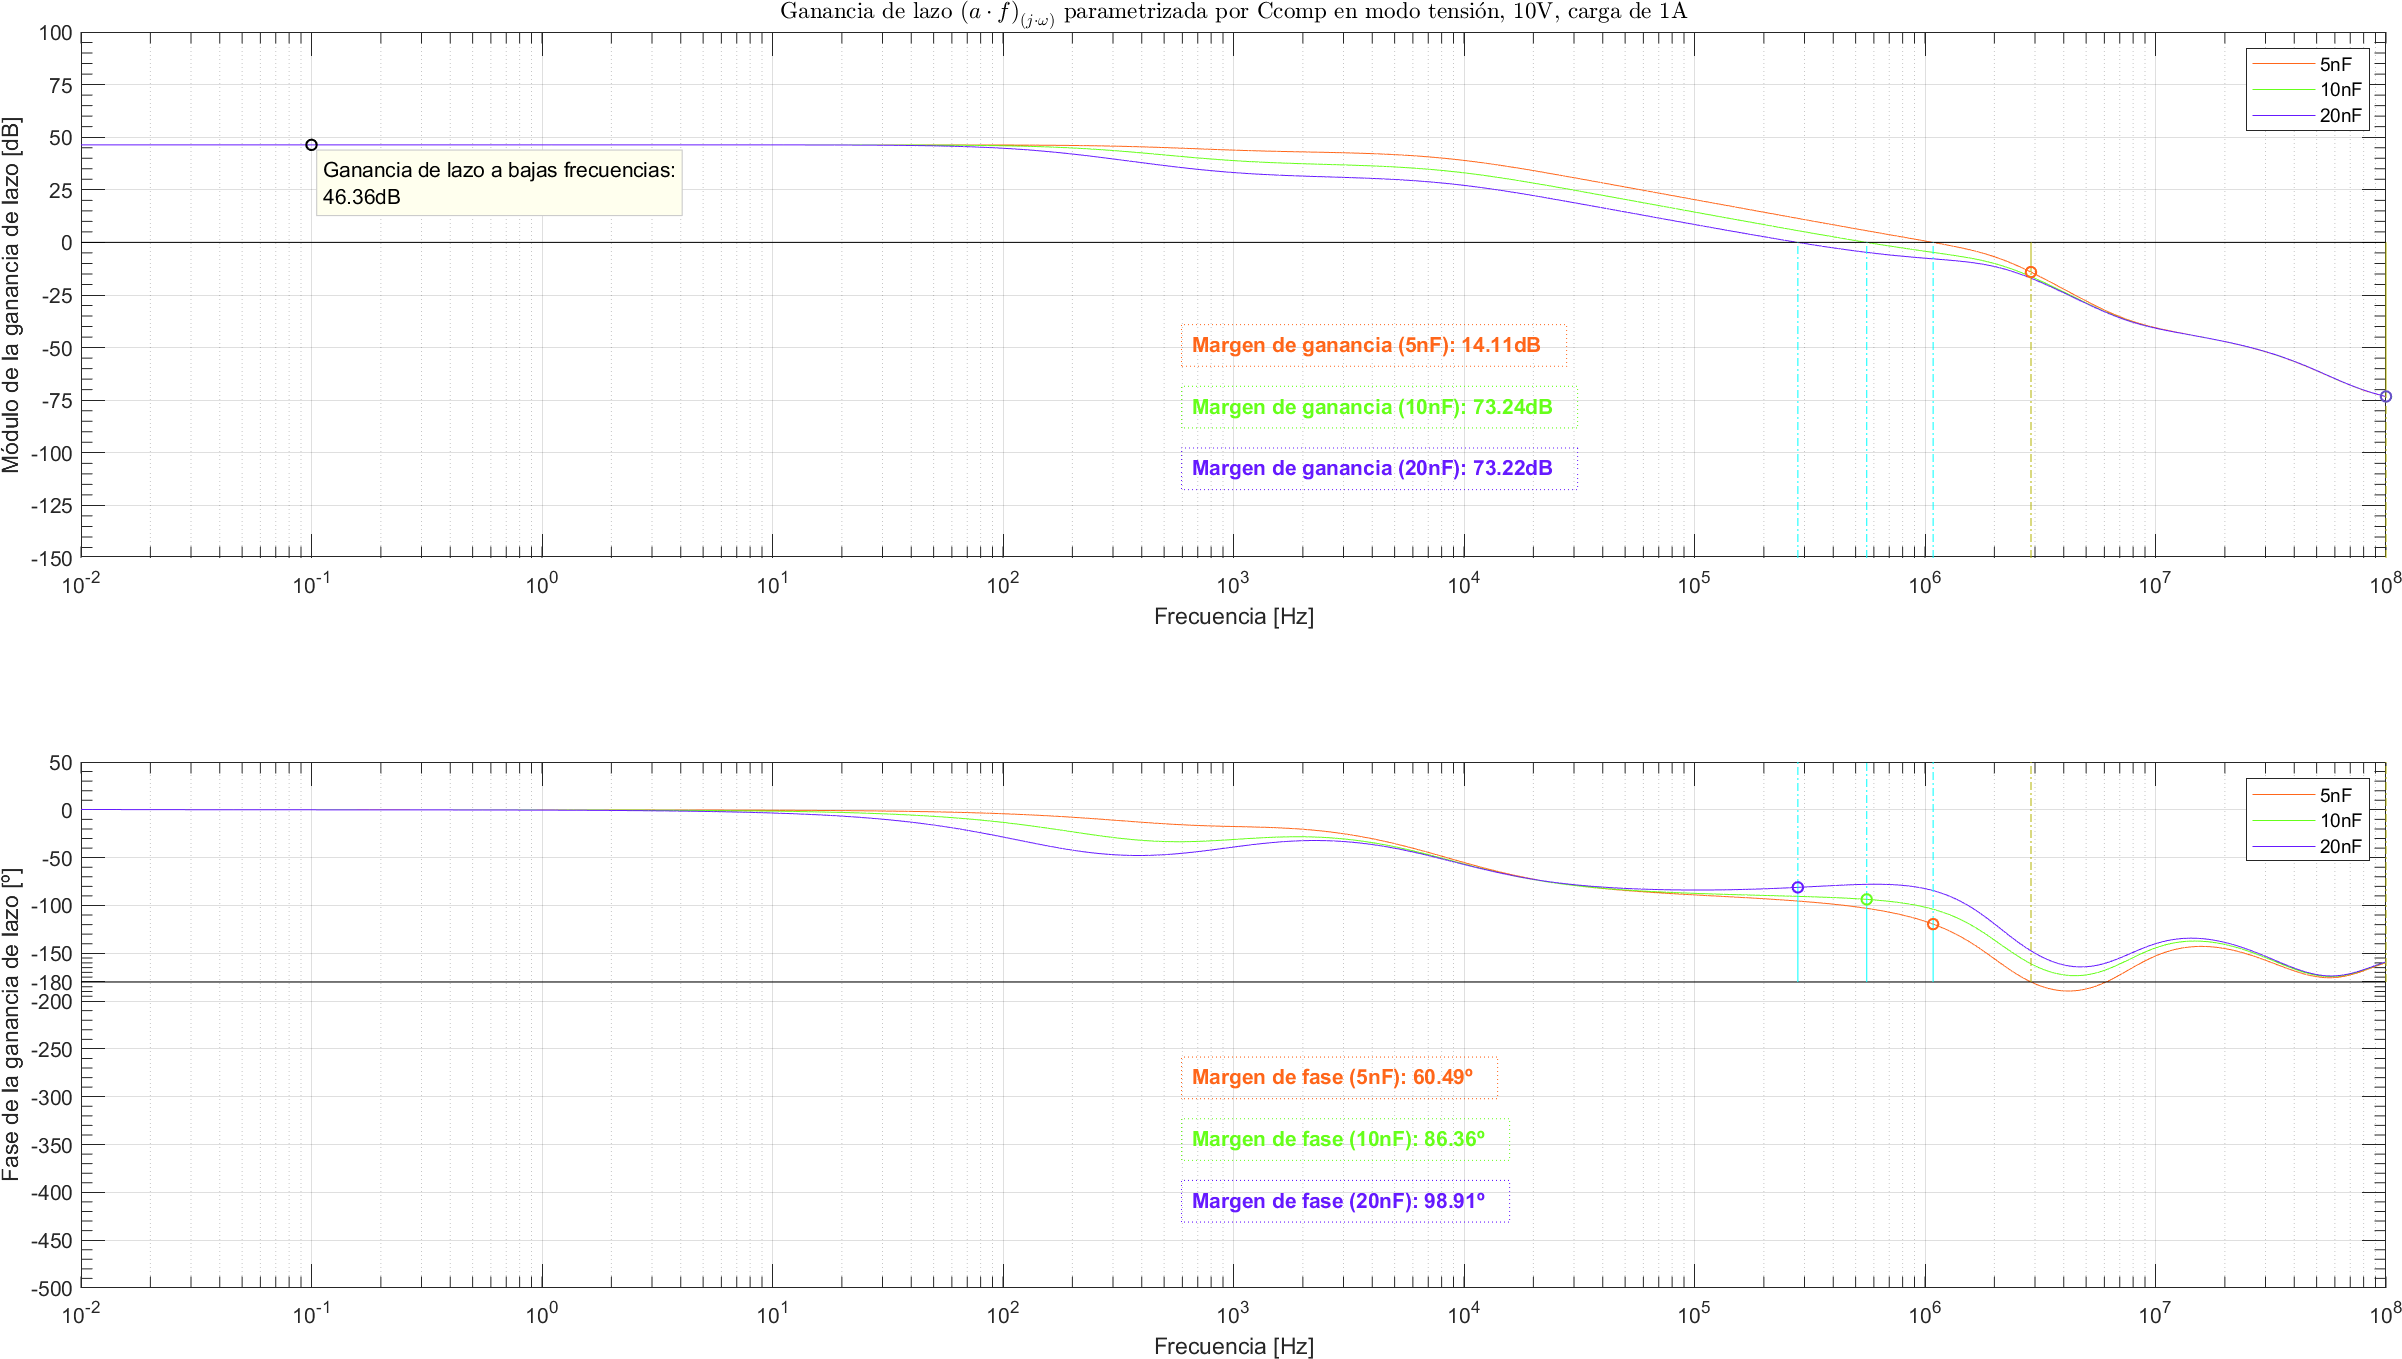
\includegraphics[width=1.1 \textwidth, angle=90]{./img/plots/loop/power_supply_CCOMP_LOOP_Modo1.png}
\caption{\label{fig:fig_power_supply_CCOMP_LOOP_Modo1}\footnotesize{Ganancia de lazo en modo tensión, $V_{out} = 10 \si[per-mode=symbol]{\volt}$, en función de la frecuencia parametrizada por $C_{comp}$.}}
\end{center}
\end{figure}


\clearpage

\begin{figure}[H] %htb
\begin{center}
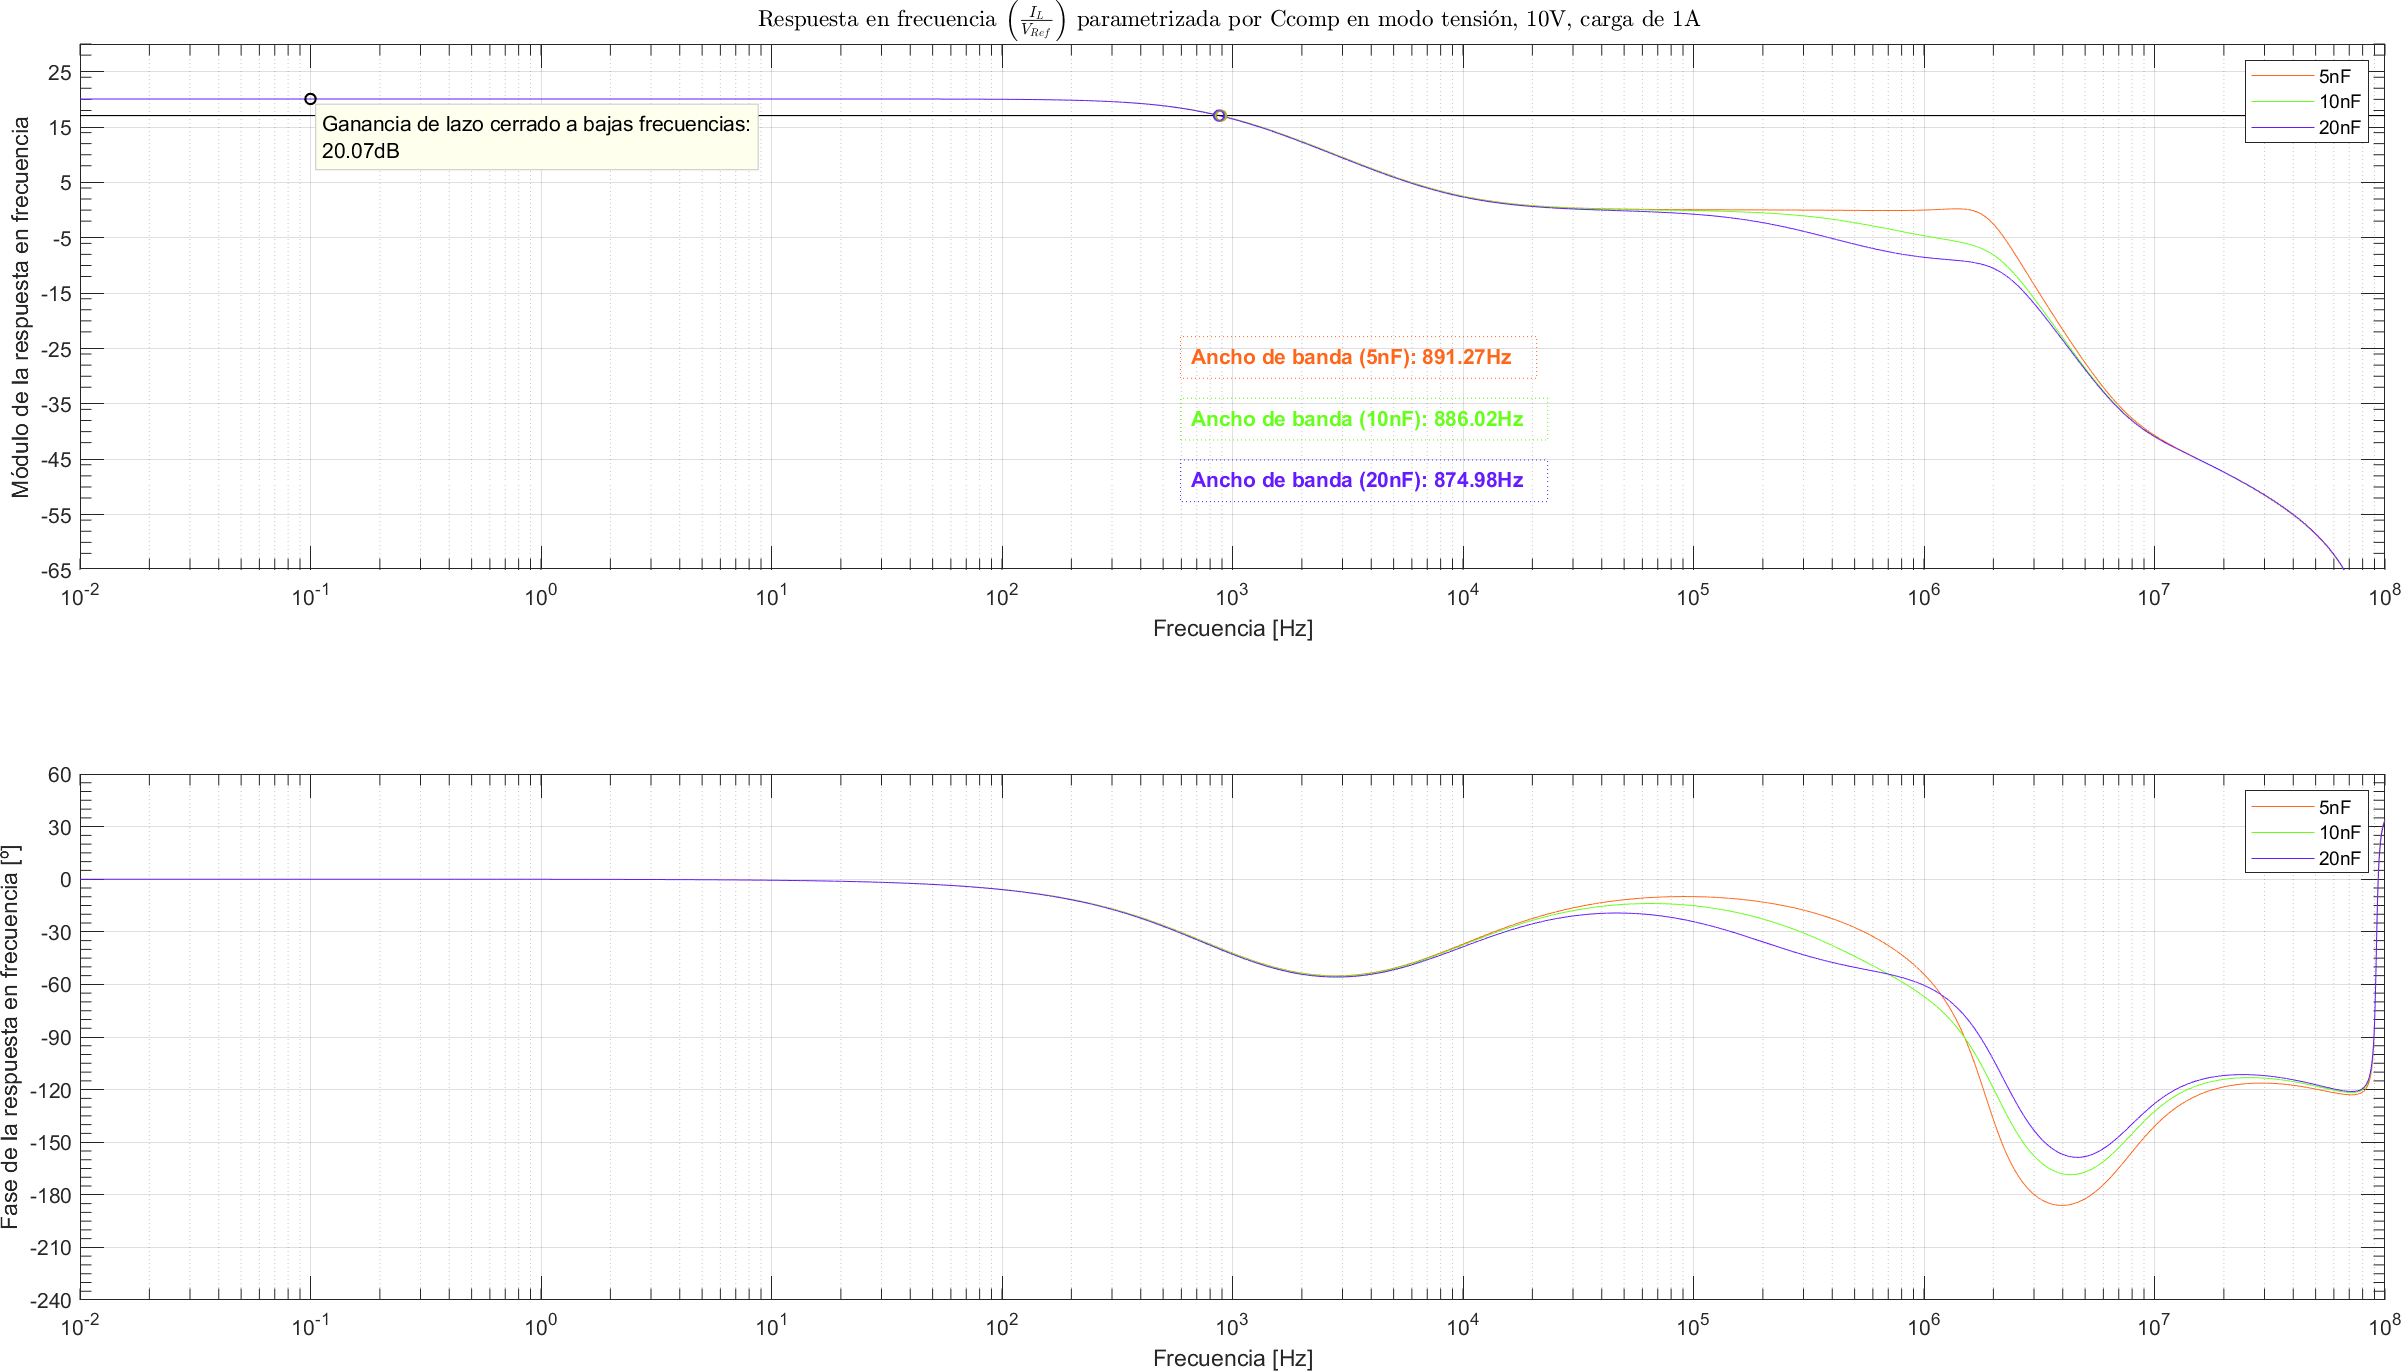
\includegraphics[width=1.1 \textwidth, angle=90]{./img/plots/rf/power_supply_CCOMP_RF_Modo1.png}
\caption{\label{fig:fig_power_supply_CCOMP_RF_Modo1}\footnotesize{Respuesta en frecuencia en modo tensión, $V_{out} = 10 \si[per-mode=symbol]{\volt}$, en función de la frecuencia parametrizada por $C_{comp}$.}}
\end{center}
\end{figure}

\clearpage

\begin{figure}[H] %htb
\begin{center}
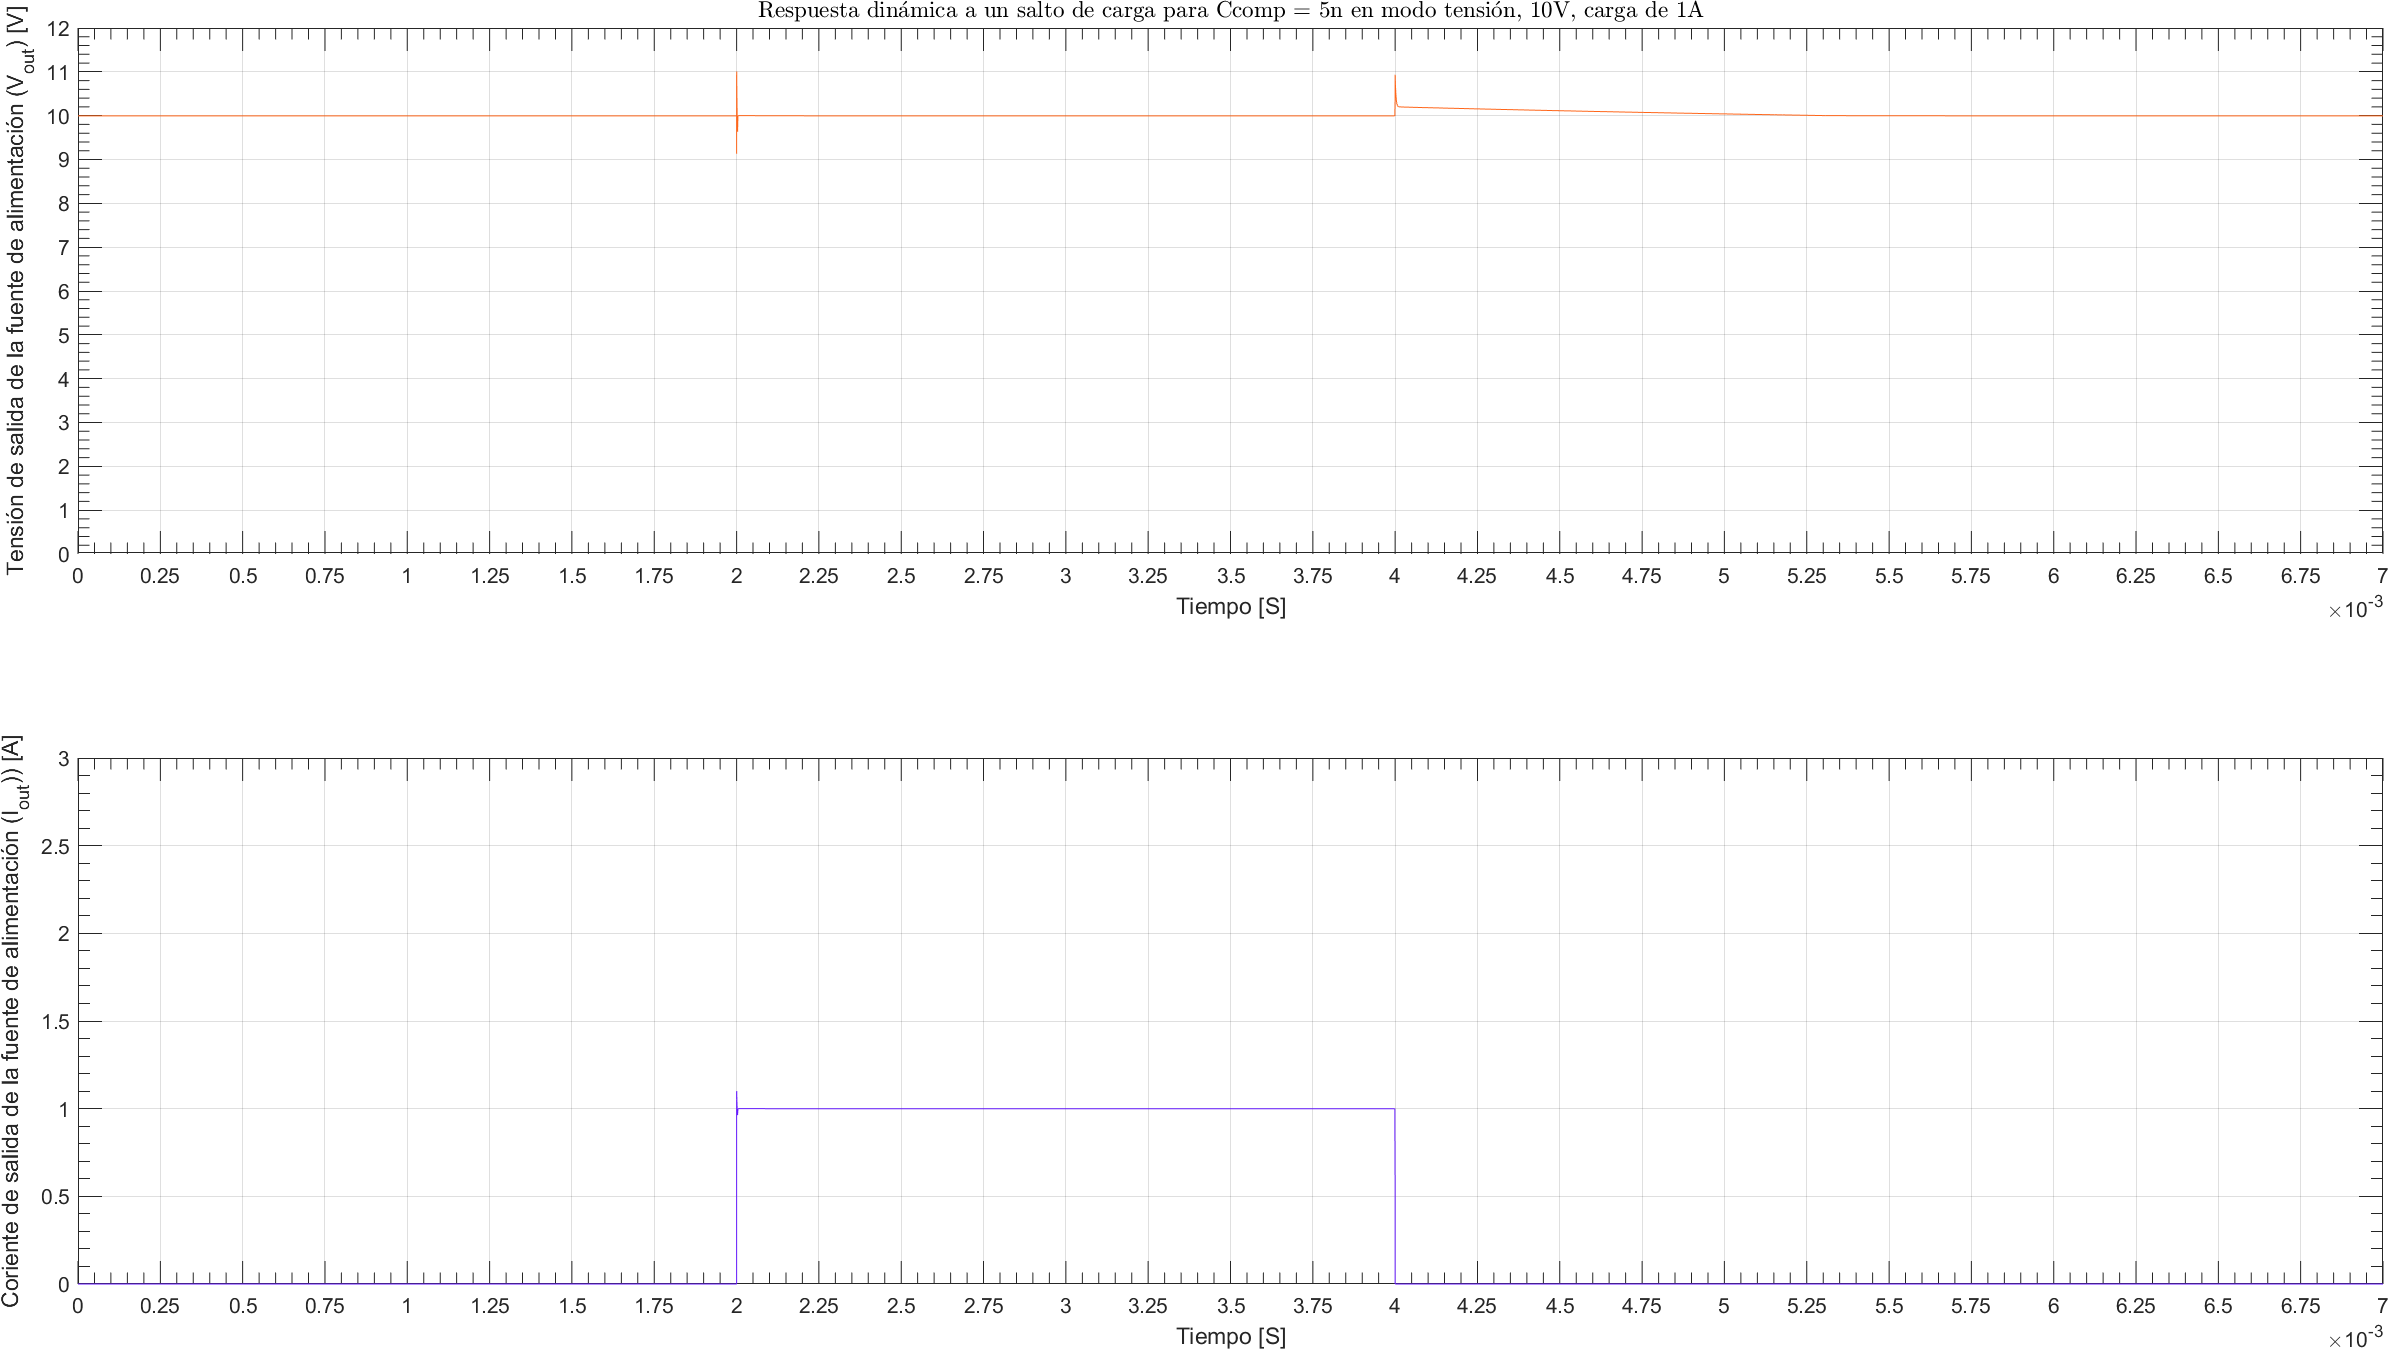
\includegraphics[width=1.1 \textwidth, angle=90]{./img/plots/dynamic/power_supply_CCOMP_5n_STEP_Modo1.png}
\caption{\label{fig:fig_power_supply_CCOMP_STEP_5n_Modo1}\footnotesize{Respuesta dinámica en modo tensión, $V_{out} = 10 \si[per-mode=symbol]{\volt}$, para $C_{comp} = 5 \si[per-mode=symbol]{\nano\farad} $.}}
\end{center}
\end{figure}

\clearpage

\begin{figure}[H] %htb
\begin{center}
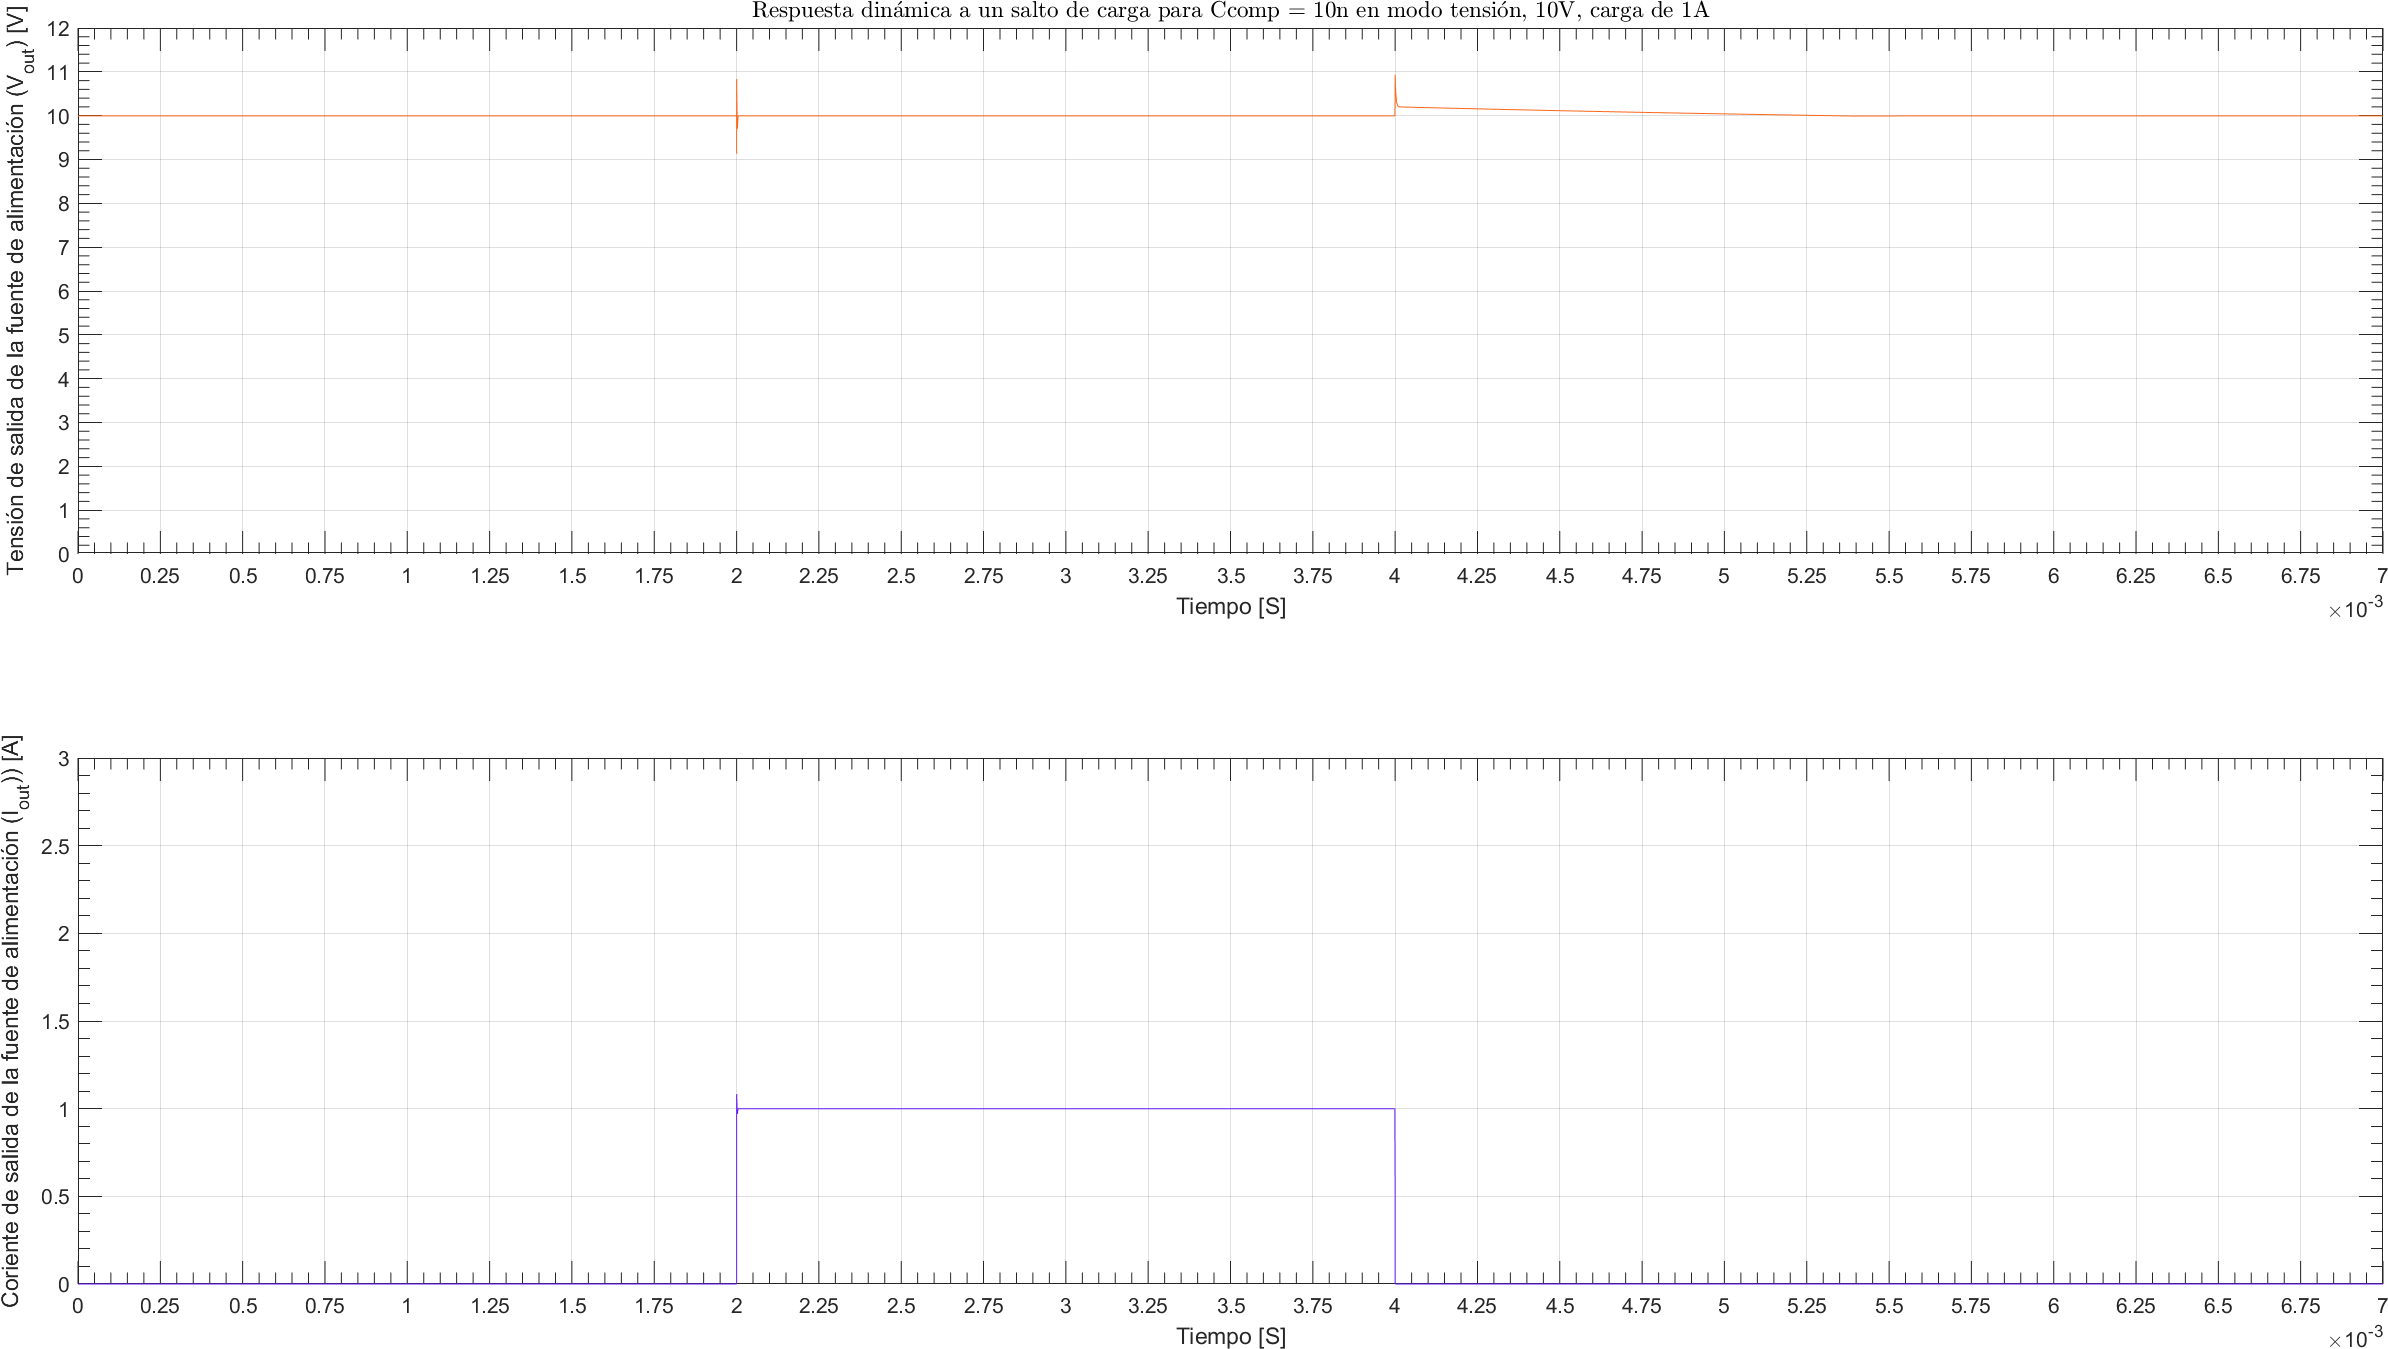
\includegraphics[width=1.1 \textwidth, angle=90]{./img/plots/dynamic/power_supply_CCOMP_10n_STEP_Modo1.png}
\caption{\label{fig:fig_power_supply_CCOMP_STEP_10n_Modo1}\footnotesize{Respuesta dinámica en modo tensión, $V_{out} = 10 \si[per-mode=symbol]{\volt}$, para $C_{comp} = 10 \si[per-mode=symbol]{\nano\farad} $.}}
\end{center}
\end{figure}

\clearpage

\begin{figure}[H] %htb
\begin{center}
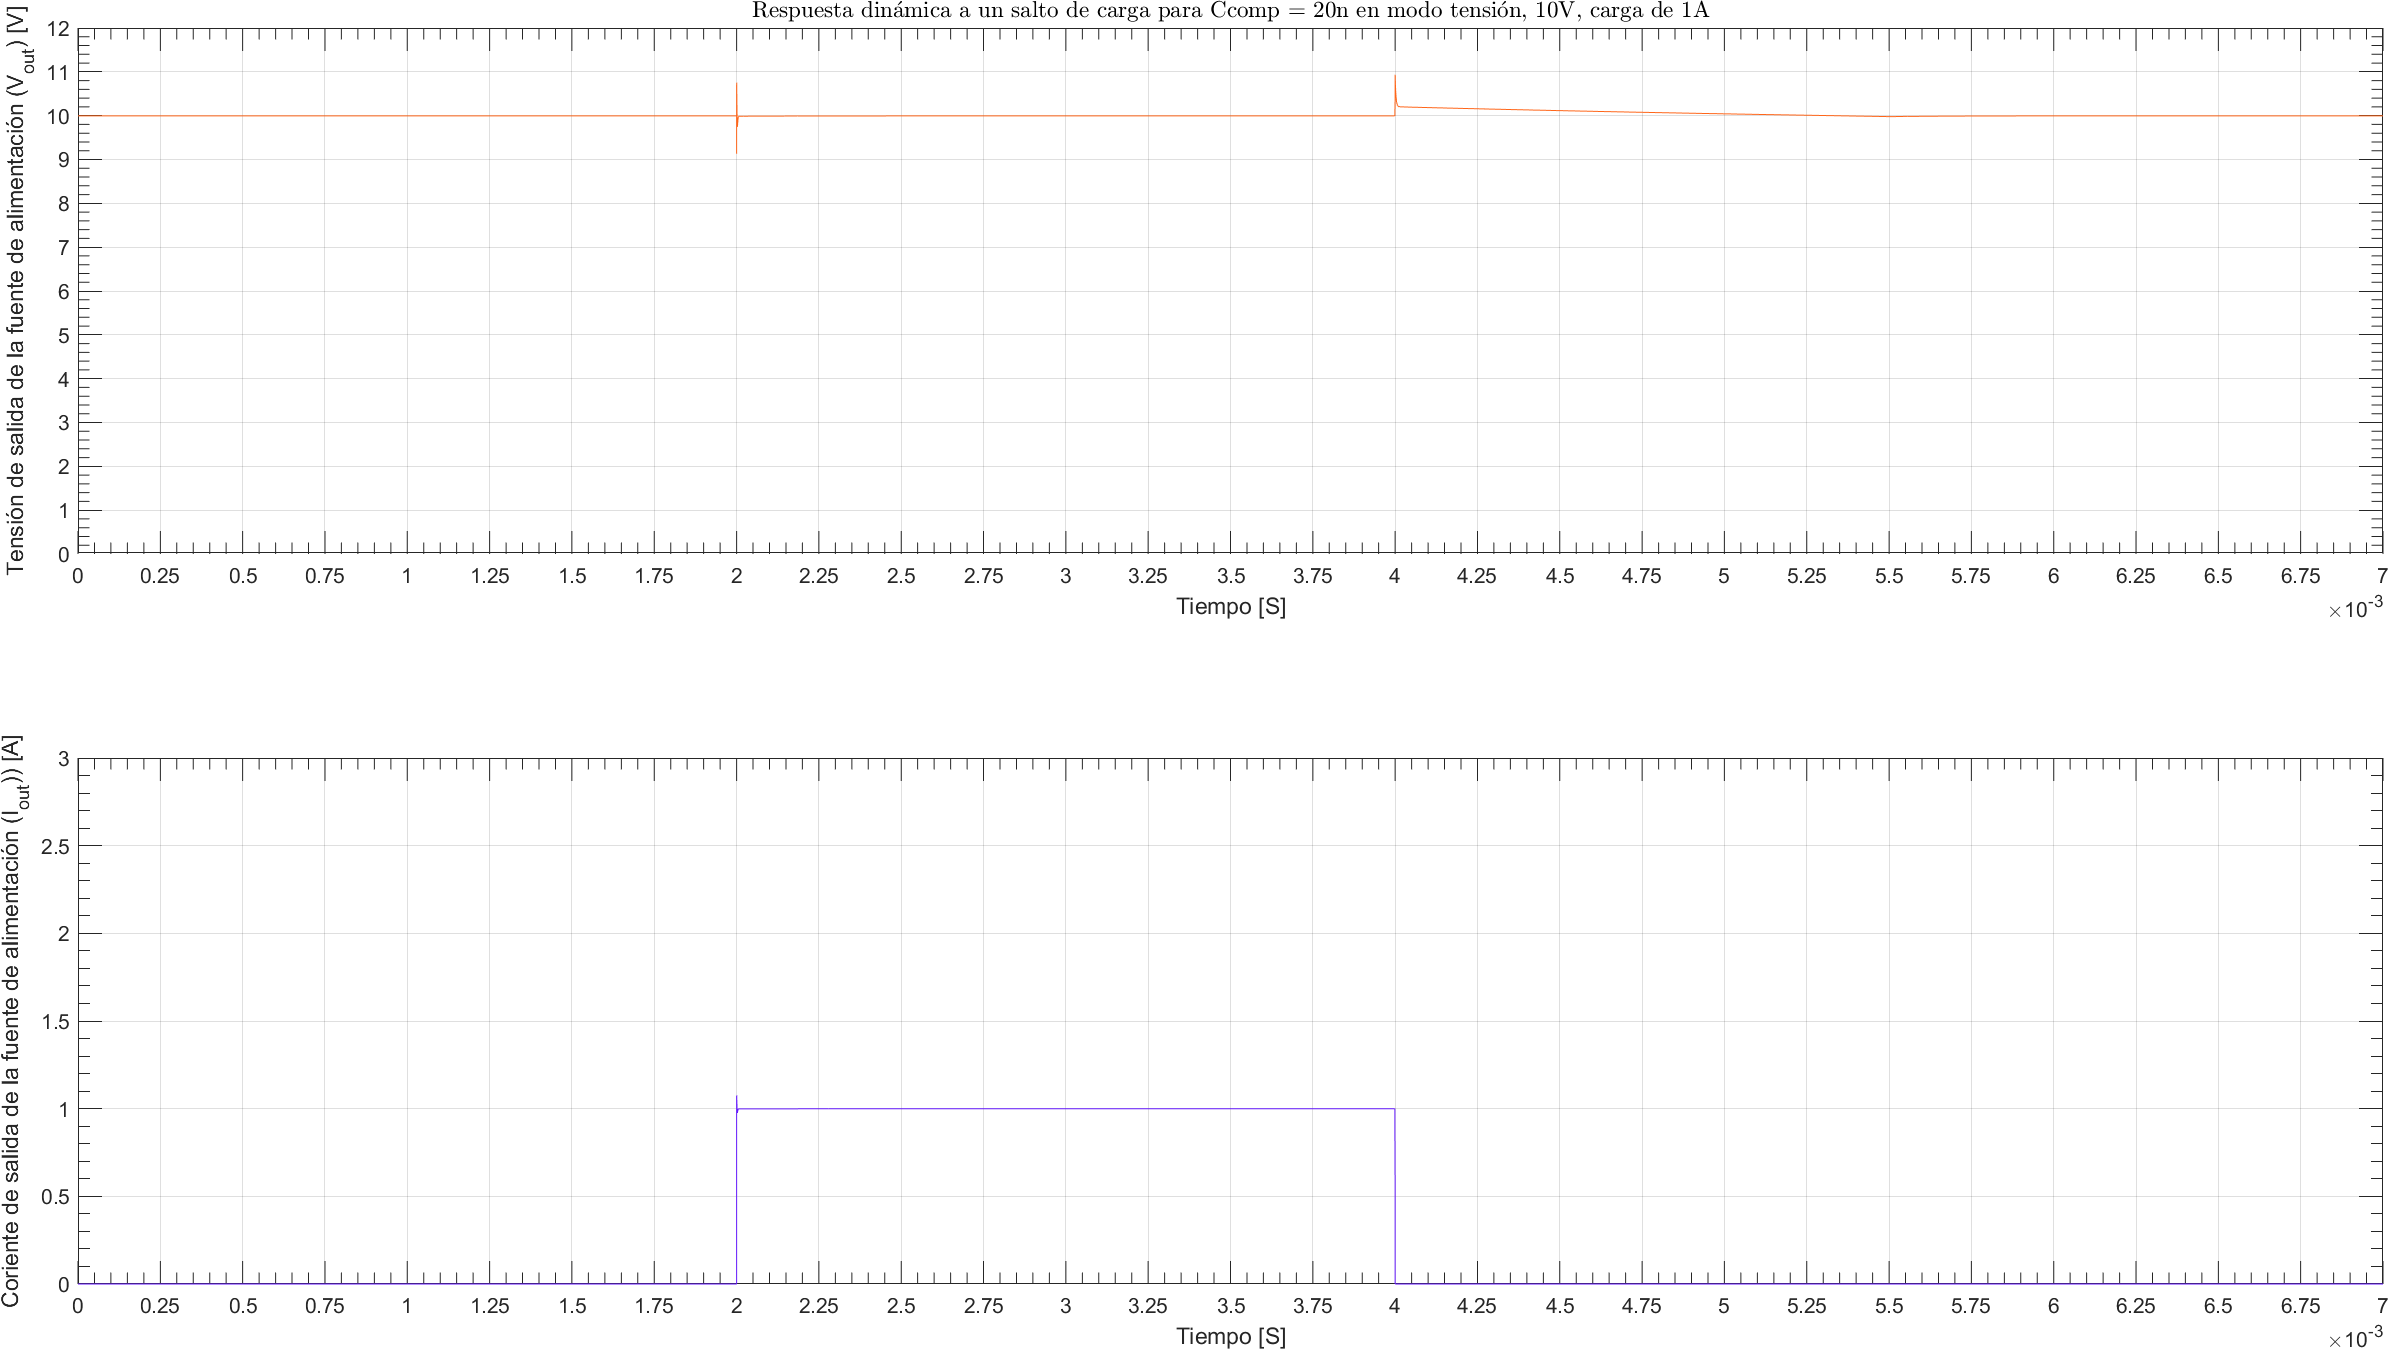
\includegraphics[width=1.1 \textwidth, angle=90]{./img/plots/dynamic/power_supply_CCOMP_20n_STEP_Modo1.png}
\caption{\label{fig:fig_power_supply_CCOMP_STEP_20n_Modo1}\footnotesize{Respuesta dinámica en modo tensión, $V_{out} = 10 \si[per-mode=symbol]{\volt}$, para $C_{comp} = 20 \si[per-mode=symbol]{\nano\farad} $.}}
\end{center}
\end{figure}

\clearpage


\subsubsection{Análisis para $C_{comp}$ en modo tensión, $V_{out} = 1 \si[per-mode=symbol]{\volt}$, $R_{L} = 1 \si[per-mode=symbol]{\ohm}$}

En forma similar al modo anterior, se puede ver en la figura~\figref{fig:fig_power_supply_CCOMP_LOOP_Modo2} como ya con el valor de $C_{comp} = 10 \si[per-mode=symbol]{\nano\farad}$ se logra unos márgenes de fase y ganancia aceptables, seguir aumentando el valor de $C_{comp}$, solo disminuye innecesariamente el ancho de banda, como se puede ver en la figura~\figref{fig:fig_power_supply_CCOMP_RF_Modo2}. A nivel de respuesta dinámica, nuevamente no se ven grandes diferencias entre los valores simulados, ver figura~\figref{fig:fig_power_supply_CCOMP_STEP_5n_Modo2}, figura~\figref{fig:fig_power_supply_CCOMP_STEP_10n_Modo2} y figura~\figref{fig:fig_power_supply_CCOMP_STEP_20n_Modo2}.

\vfill


% CCOMP MODO 2.

\clearpage

\begin{figure}[H] %htb
\begin{center}
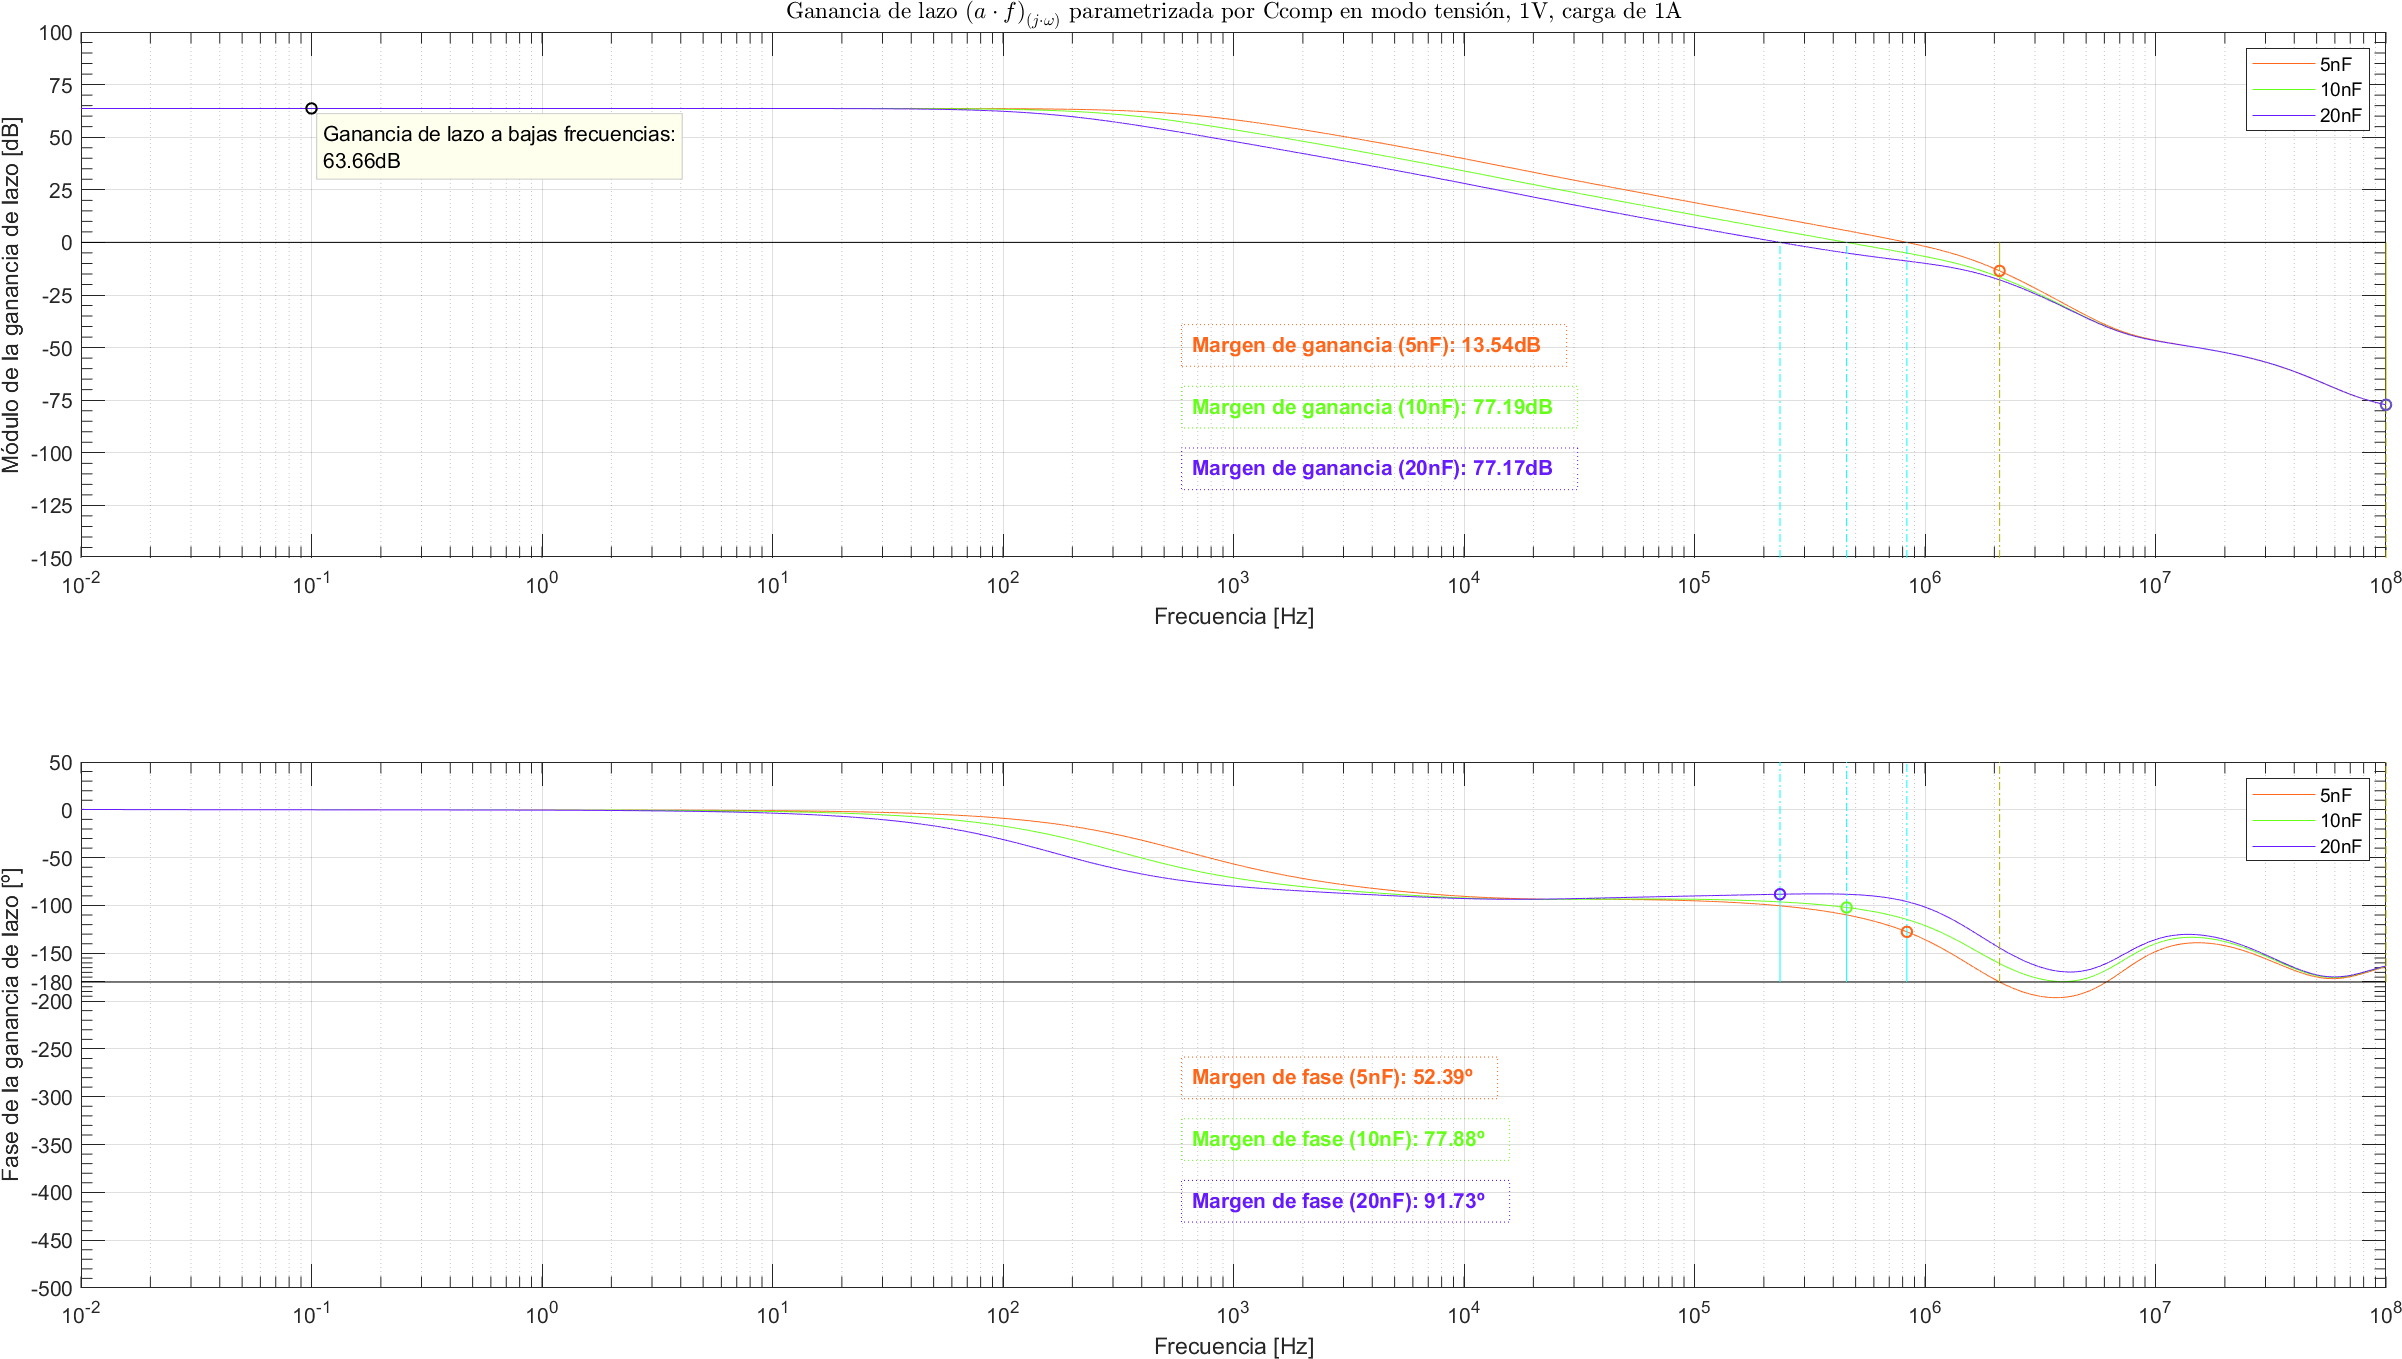
\includegraphics[width=1.1 \textwidth, angle=90]{./img/plots/loop/power_supply_CCOMP_LOOP_Modo2.png}
\caption{\label{fig:fig_power_supply_CCOMP_LOOP_Modo2}\footnotesize{Ganancia de lazo en modo tensión, $V_{out} = 1 \si[per-mode=symbol]{\volt}$, en función de la frecuencia parametrizada por $C_{comp}$.}}
\end{center}
\end{figure}


\clearpage

\begin{figure}[H] %htb
\begin{center}
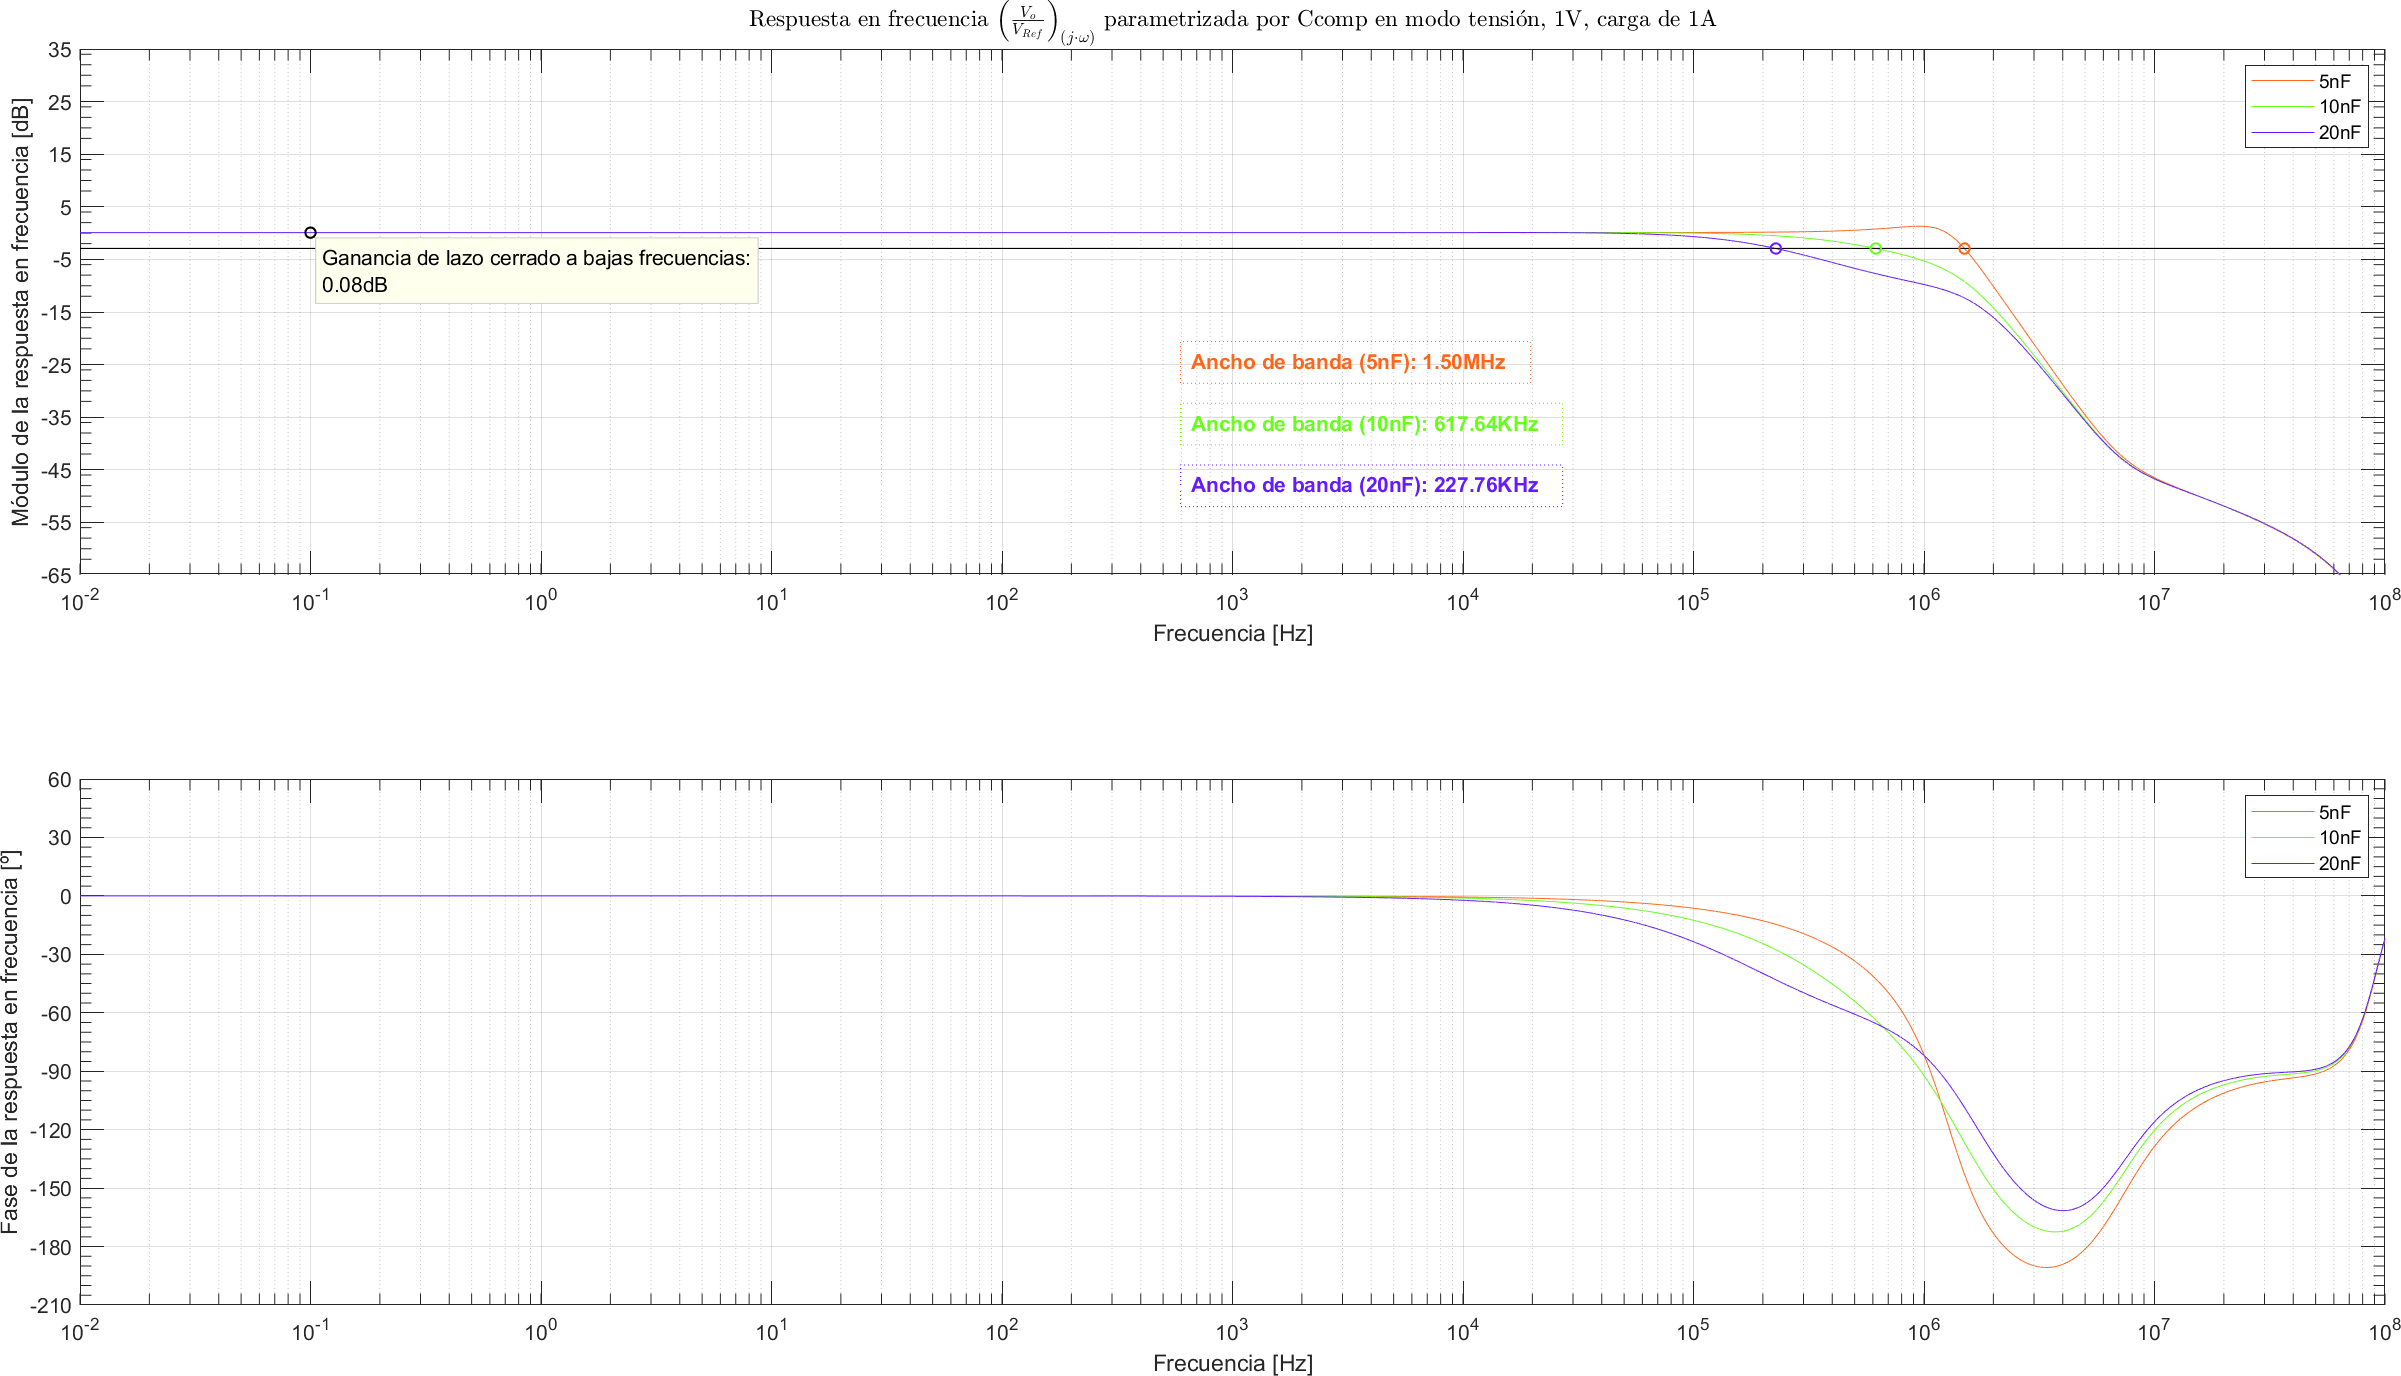
\includegraphics[width=1.1 \textwidth, angle=90]{./img/plots/rf/power_supply_CCOMP_RF_Modo2.png}
\caption{\label{fig:fig_power_supply_CCOMP_RF_Modo2}\footnotesize{Respuesta en frecuencia en modo tensión, $V_{out} = 1 \si[per-mode=symbol]{\volt}$, en función de la frecuencia parametrizada por $C_{comp}$.}}
\end{center}
\end{figure}

\clearpage

\begin{figure}[H] %htb
\begin{center}
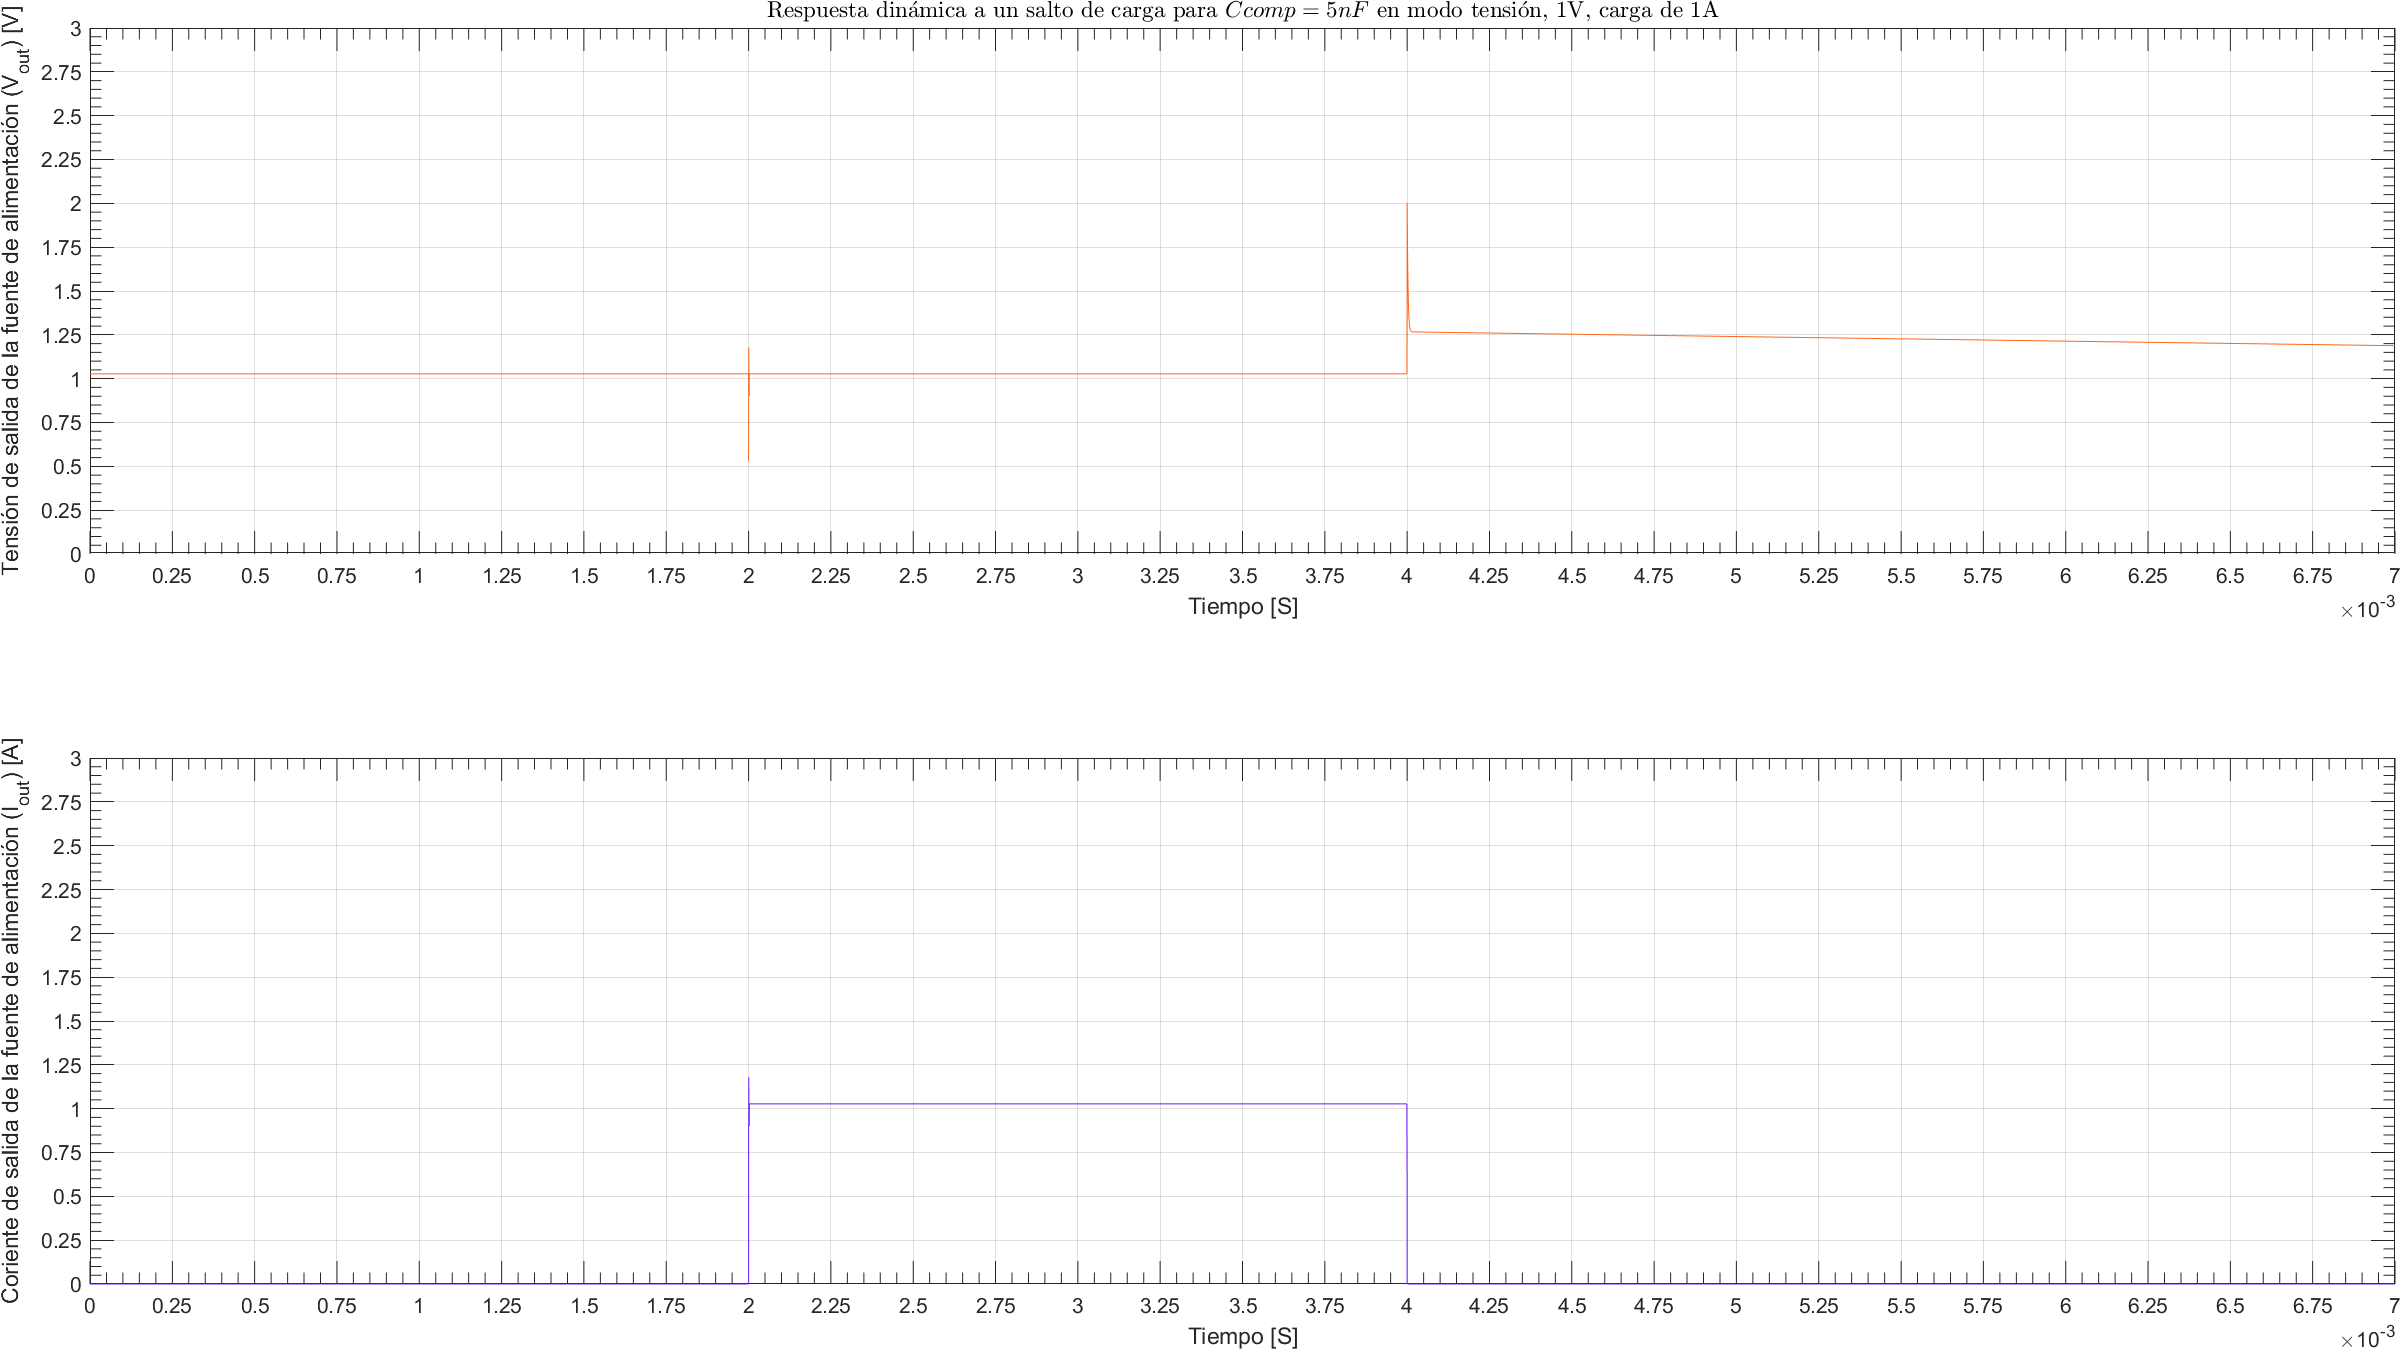
\includegraphics[width=1.1 \textwidth, angle=90]{./img/plots/dynamic/power_supply_CCOMP_5n_STEP_Modo2.png}
\caption{\label{fig:fig_power_supply_CCOMP_STEP_5n_Modo2}\footnotesize{Respuesta dinámica en modo tensión, $V_{out} = 1 \si[per-mode=symbol]{\volt}$, para $C_{comp} = 5 \si[per-mode=symbol]{\nano\farad} $.}}
\end{center}
\end{figure}

\clearpage

\begin{figure}[H] %htb
\begin{center}
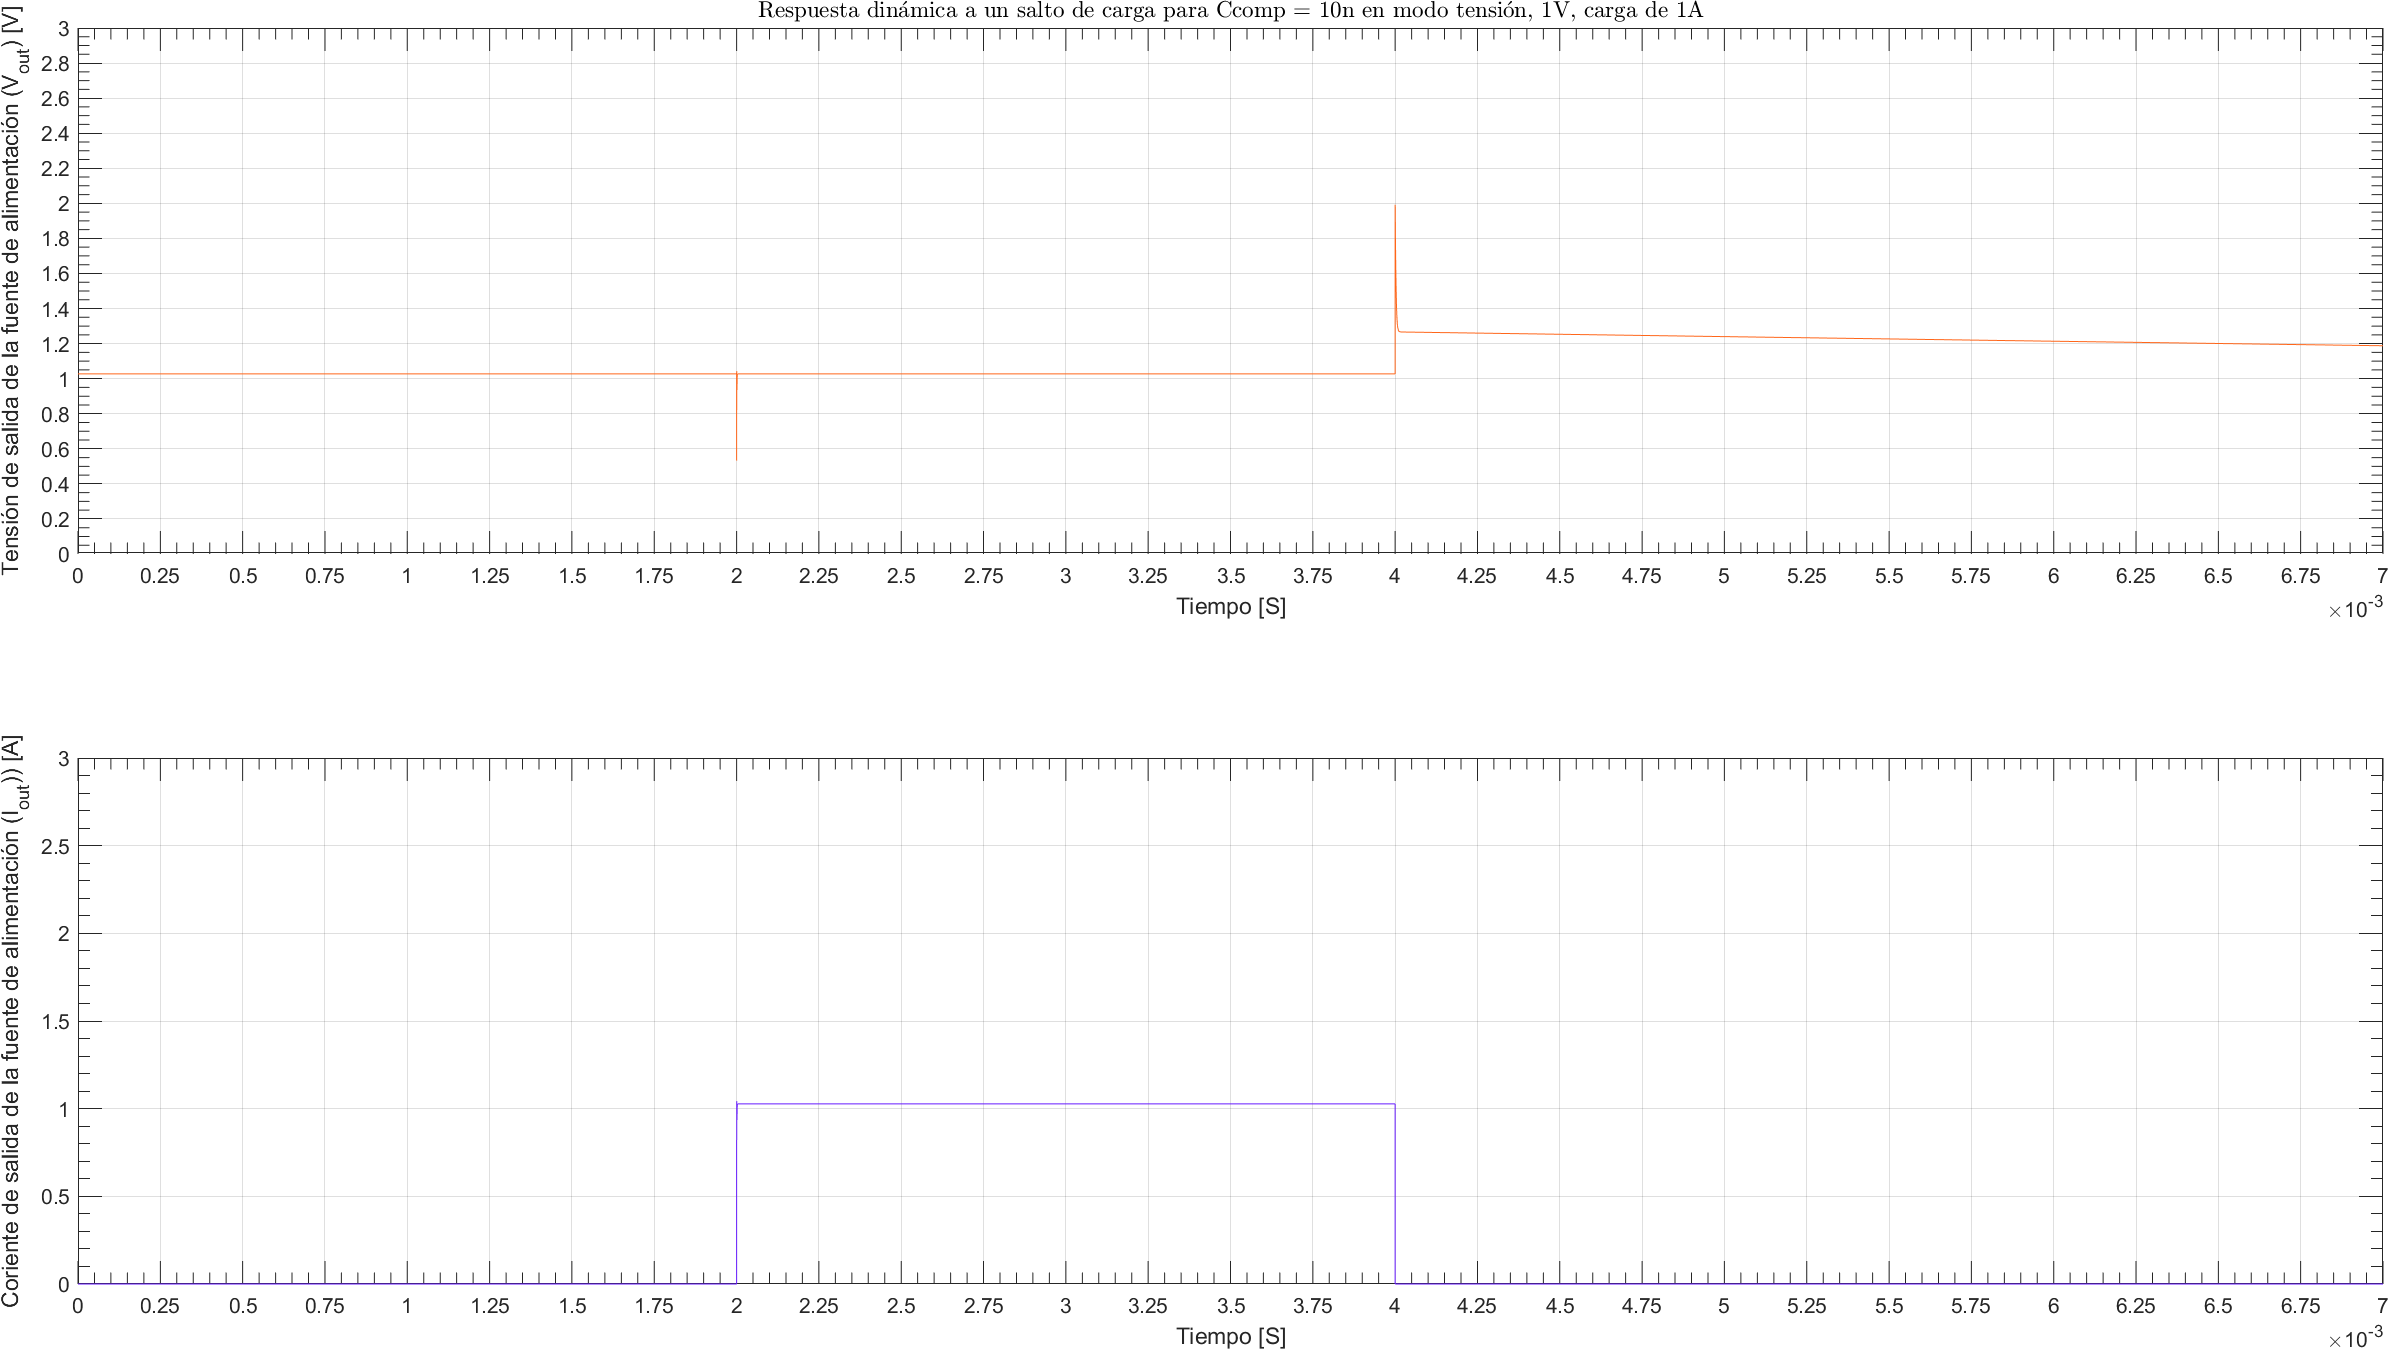
\includegraphics[width=1.1 \textwidth, angle=90]{./img/plots/dynamic/power_supply_CCOMP_10n_STEP_Modo2.png}
\caption{\label{fig:fig_power_supply_CCOMP_STEP_10n_Modo2}\footnotesize{Respuesta dinámica en modo tensión, $V_{out} = 1 \si[per-mode=symbol]{\volt}$, para $C_{comp} = 10 \si[per-mode=symbol]{\nano\farad} $.}}
\end{center}
\end{figure}

\clearpage

\begin{figure}[H] %htb
\begin{center}
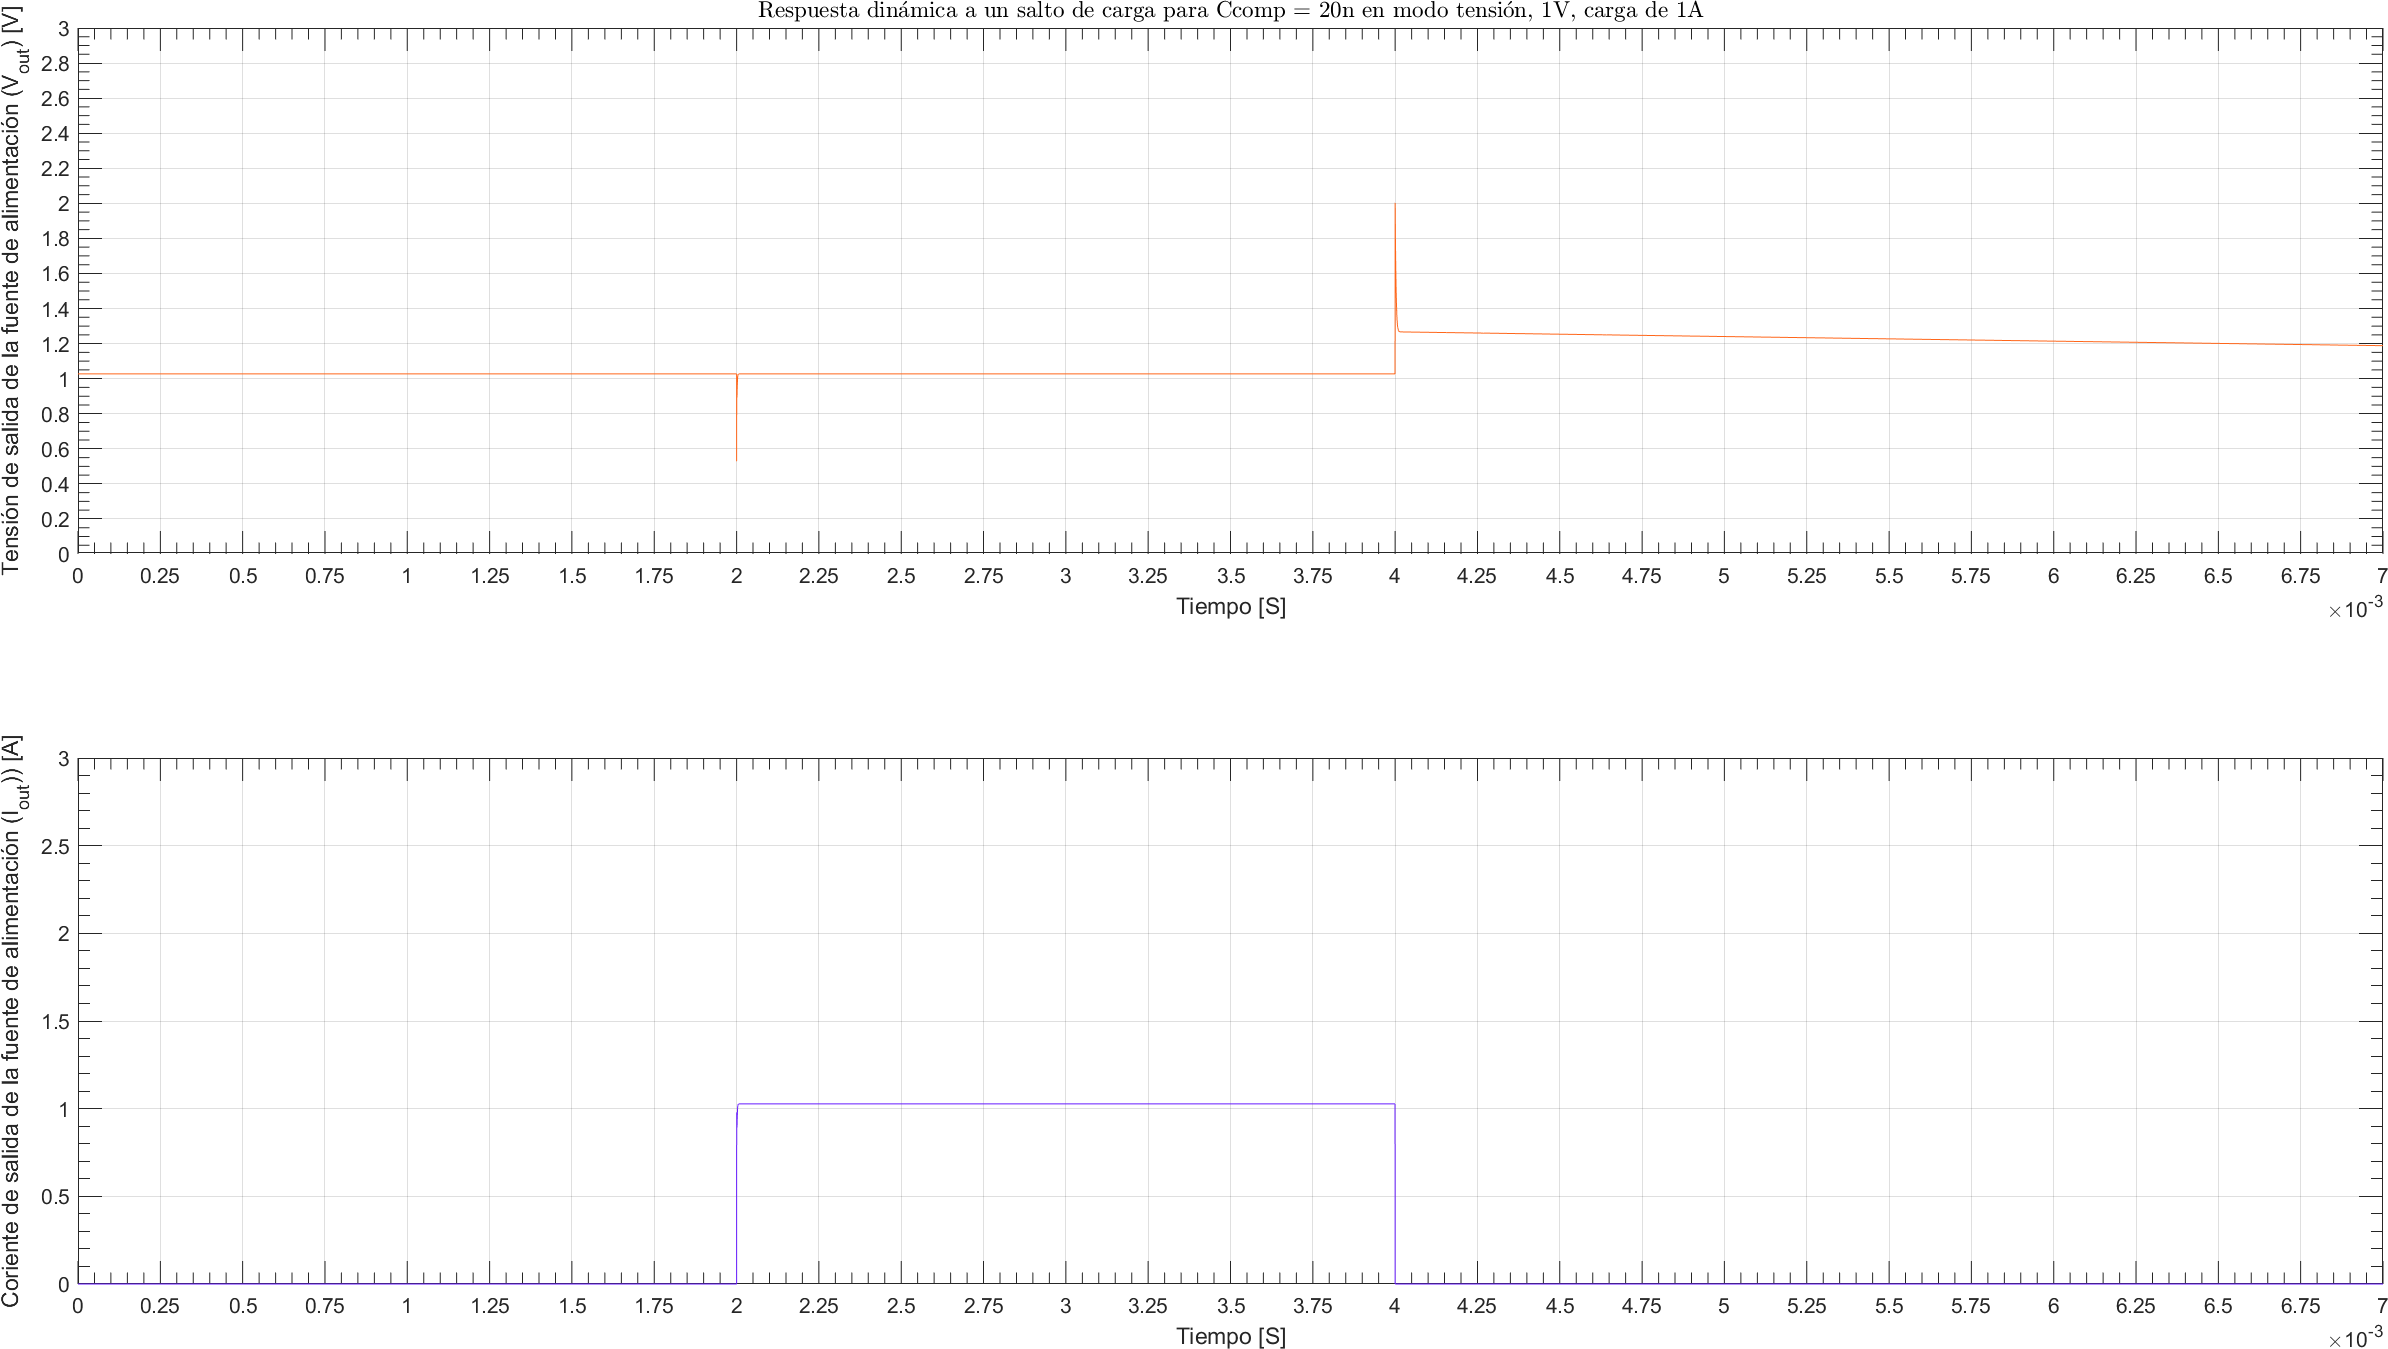
\includegraphics[width=1.1 \textwidth, angle=90]{./img/plots/dynamic/power_supply_CCOMP_20n_STEP_Modo2.png}
\caption{\label{fig:fig_power_supply_CCOMP_STEP_20n_Modo2}\footnotesize{Respuesta dinámica en modo tensión, $V_{out} = 1 \si[per-mode=symbol]{\volt}$, para $C_{comp} = 20 \si[per-mode=symbol]{\nano\farad} $.}}
\end{center}
\end{figure}

\clearpage


\subsubsection{Análisis para $C_{comp}$ en modo corriente, $I_{out} = 2 \si[per-mode=symbol]{\ampere}$, $R_{L} = 0 \si[per-mode=symbol]{\ohm}$}

En forma similar al modo anterior, se puede ver en la figura~\figref{fig:fig_power_supply_CCOMP_LOOP_Modo3} como ya con el valor de $C_{comp} = 10 \si[per-mode=symbol]{\nano\farad}$ se logra unos márgenes de fase y ganancia aceptables, seguir aumentando el valor de $C_{comp}$, solo disminuye innecesariamente el ancho de banda, como se puede ver en la figura~\figref{fig:fig_power_supply_CCOMP_RF_Modo3}. A nivel de respuesta dinámica, nuevamente no se ven grandes diferencias entre los valores simulados, pero ya el tiempo de crecimiento se ve que es apreciablemte mayor que en los casos anteriores, ver figura~\figref{fig:fig_power_supply_CCOMP_STEP_5n_Modo3}, figura~\figref{fig:fig_power_supply_CCOMP_STEP_10n_Modo3} y figura~\figref{fig:fig_power_supply_CCOMP_STEP_20n_Modo3}.

\vfill


% CCOMP MODO 3.

\clearpage

\begin{figure}[H] %htb
\begin{center}
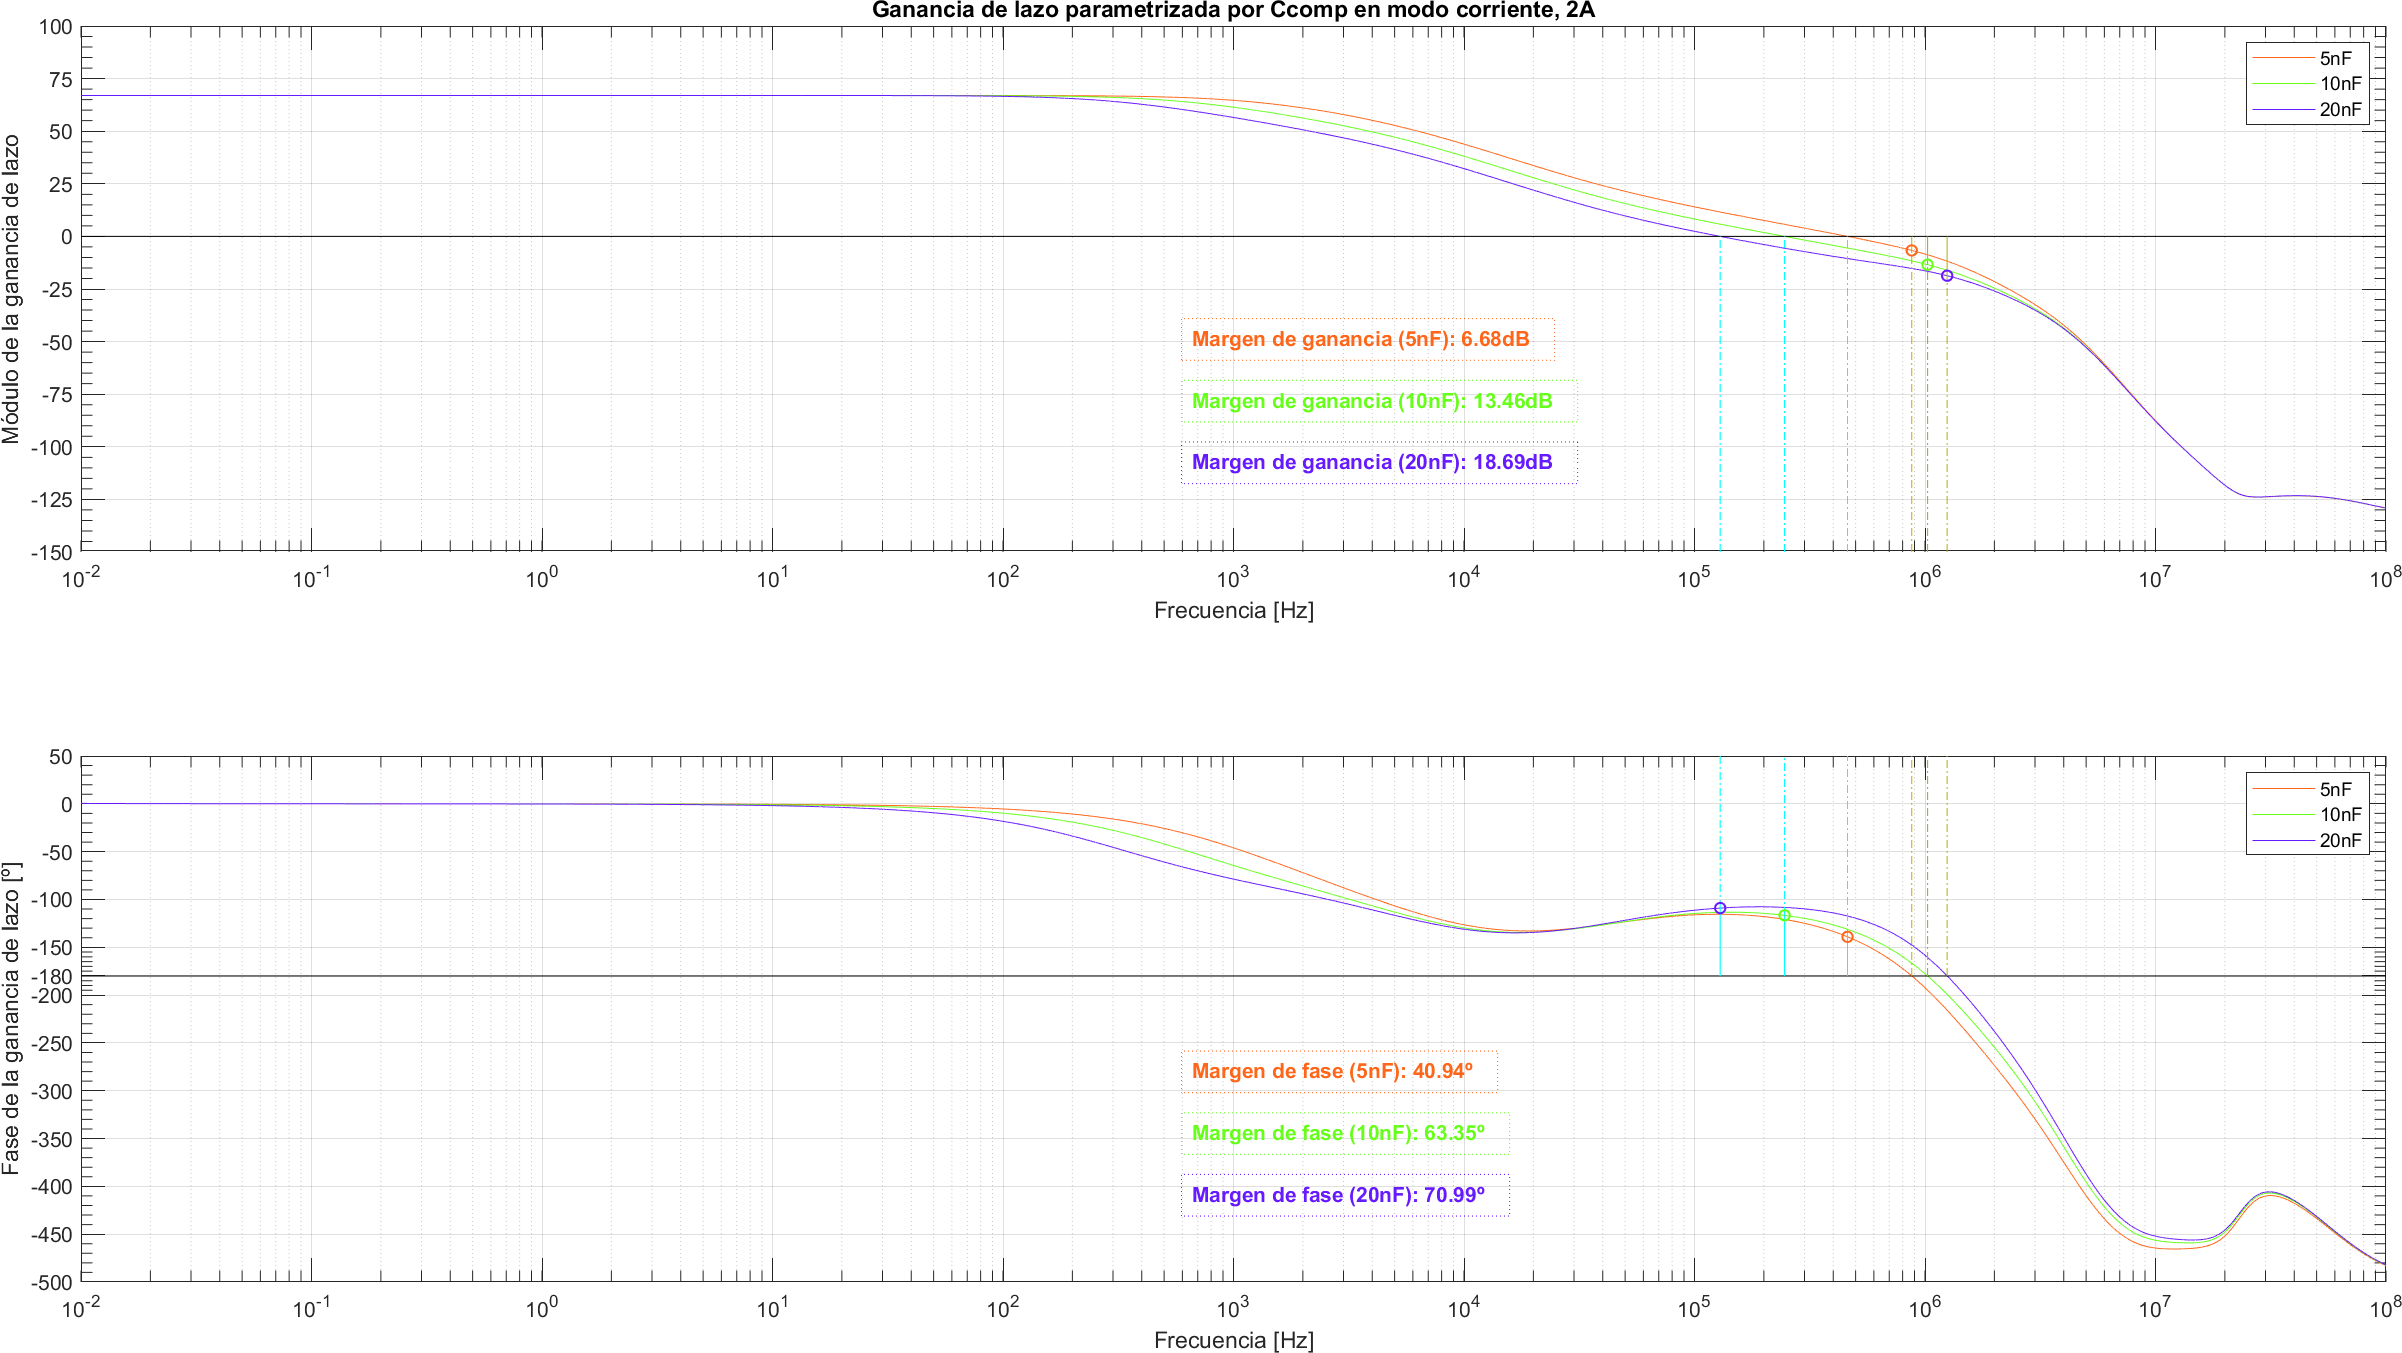
\includegraphics[width=1.1 \textwidth, angle=90]{./img/plots/loop/power_supply_CCOMP_LOOP_Modo3.png}
\caption{\label{fig:fig_power_supply_CCOMP_LOOP_Modo3}\footnotesize{Ganancia de lazo en modo corriente, $I_{out} = 2 \si[per-mode=symbol]{\ampere}$, en función de la frecuencia parametrizada por $C_{comp}$.}}
\end{center}
\end{figure}


\clearpage

\begin{figure}[H] %htb
\begin{center}
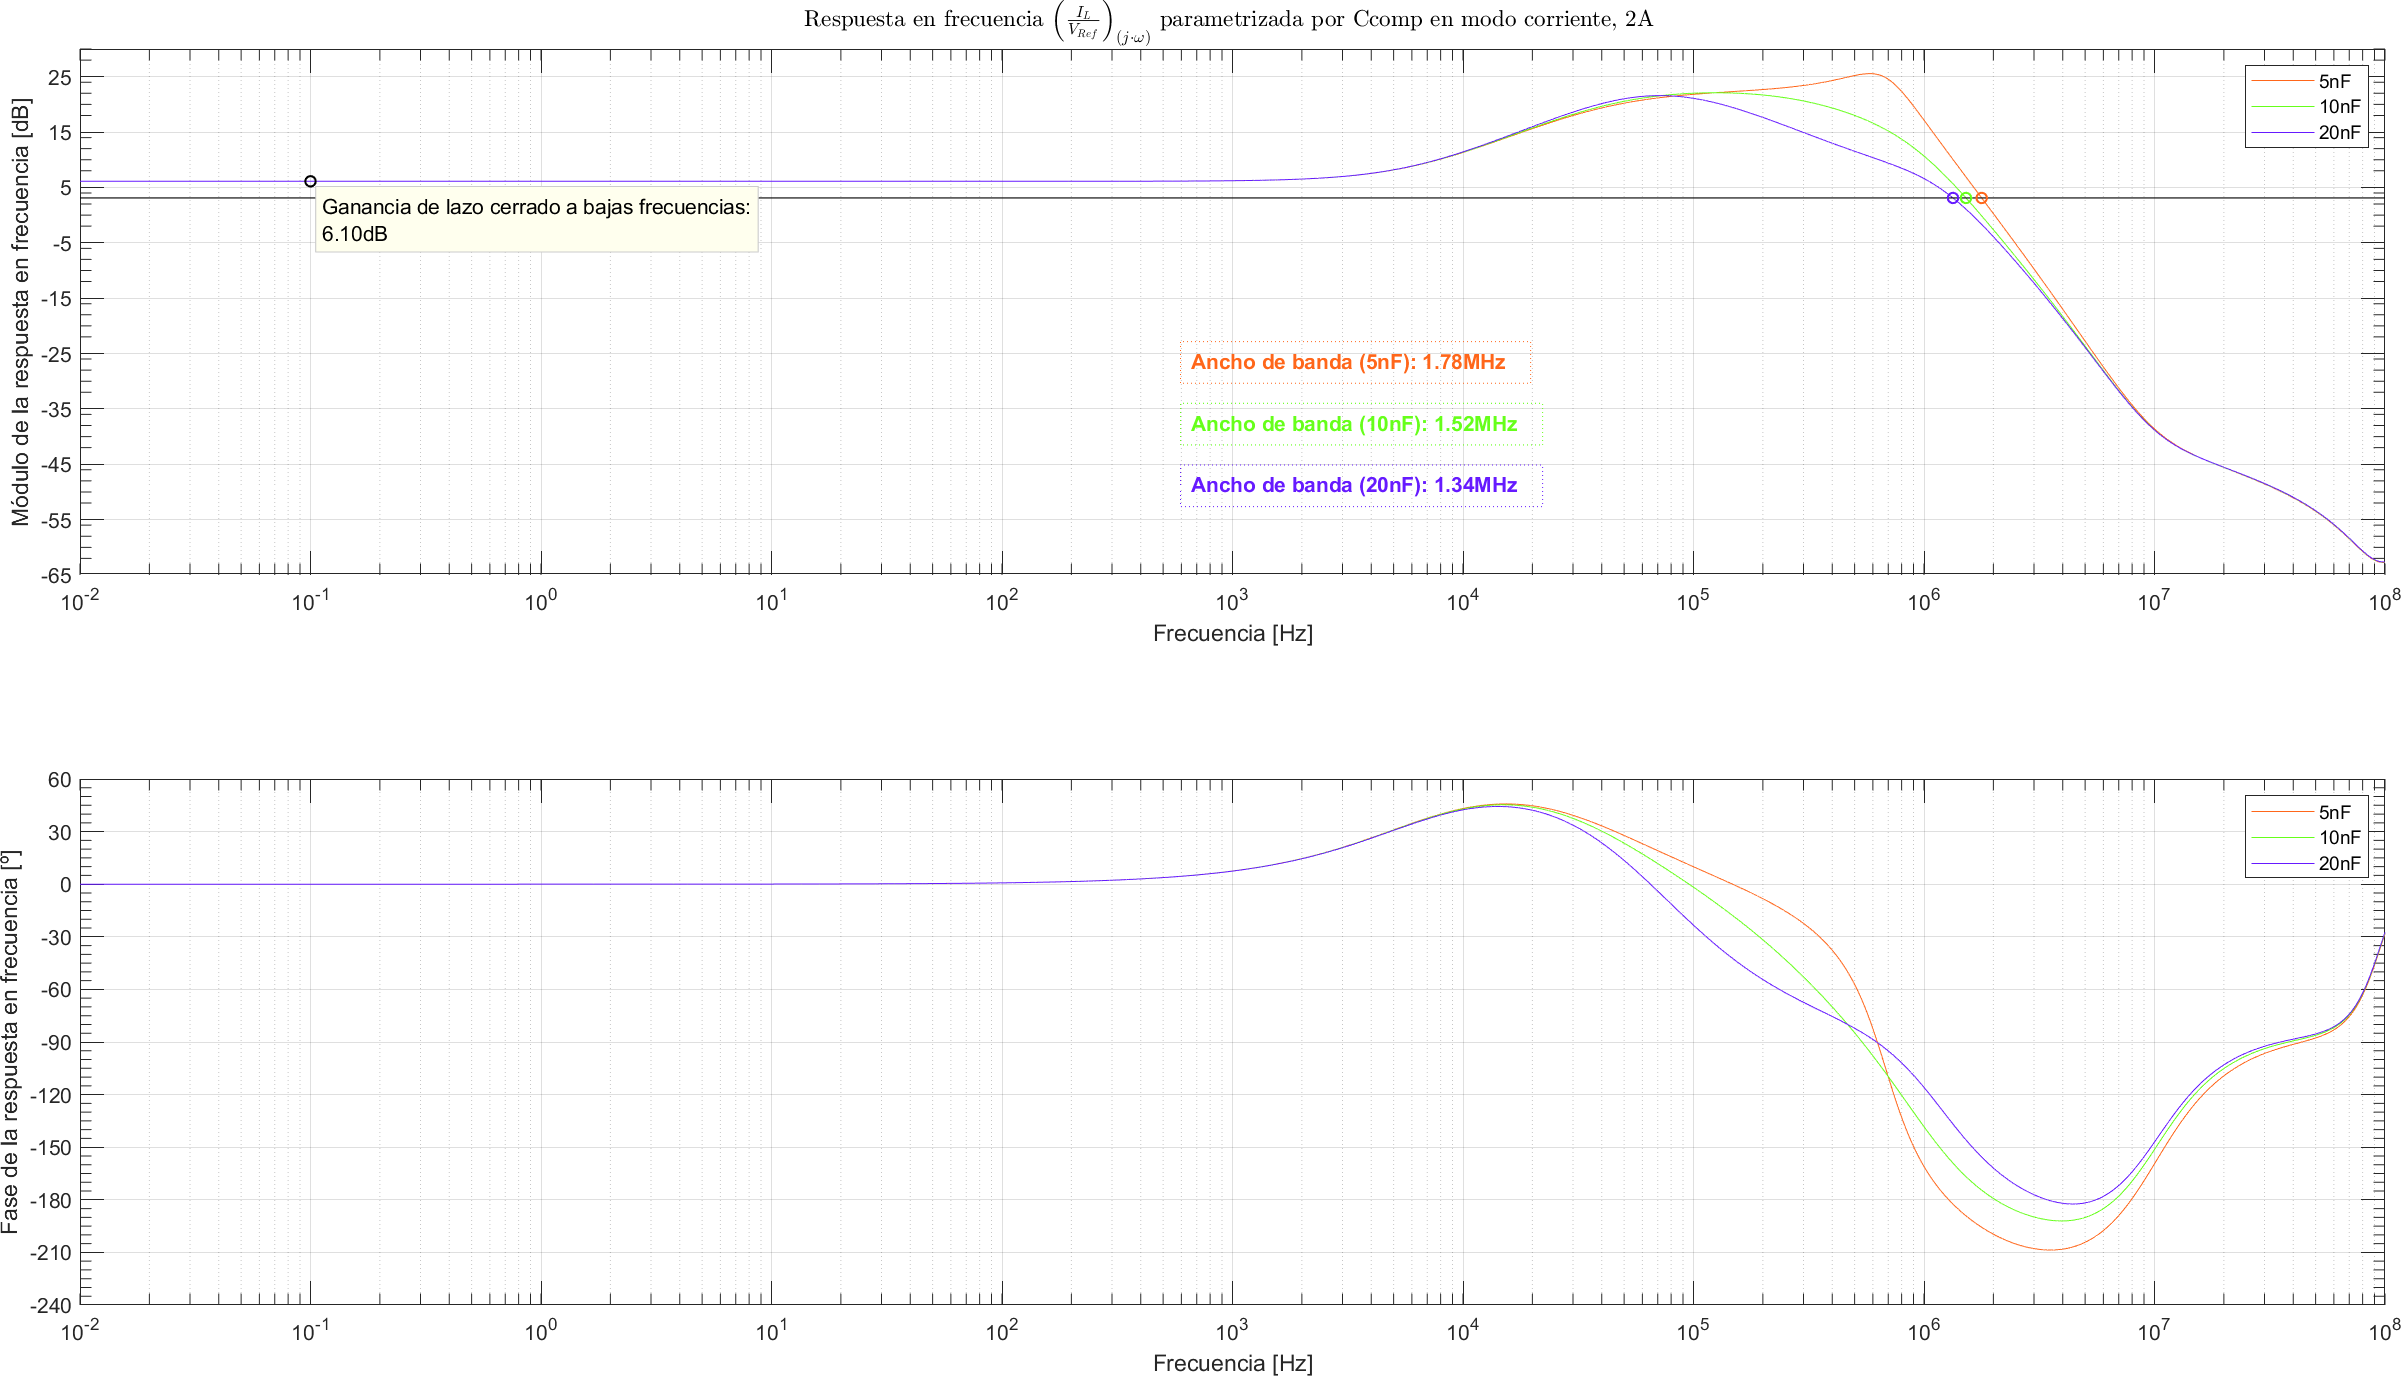
\includegraphics[width=1.1 \textwidth, angle=90]{./img/plots/rf/power_supply_CCOMP_RF_Modo3.png}
\caption{\label{fig:fig_power_supply_CCOMP_RF_Modo3}\footnotesize{Respuesta en frecuencia en modo corriente, $I_{out} = 2 \si[per-mode=symbol]{\ampere}$, en función de la frecuencia parametrizada por $C_{comp}$.}}
\end{center}
\end{figure}

\clearpage

\begin{figure}[H] %htb
\begin{center}
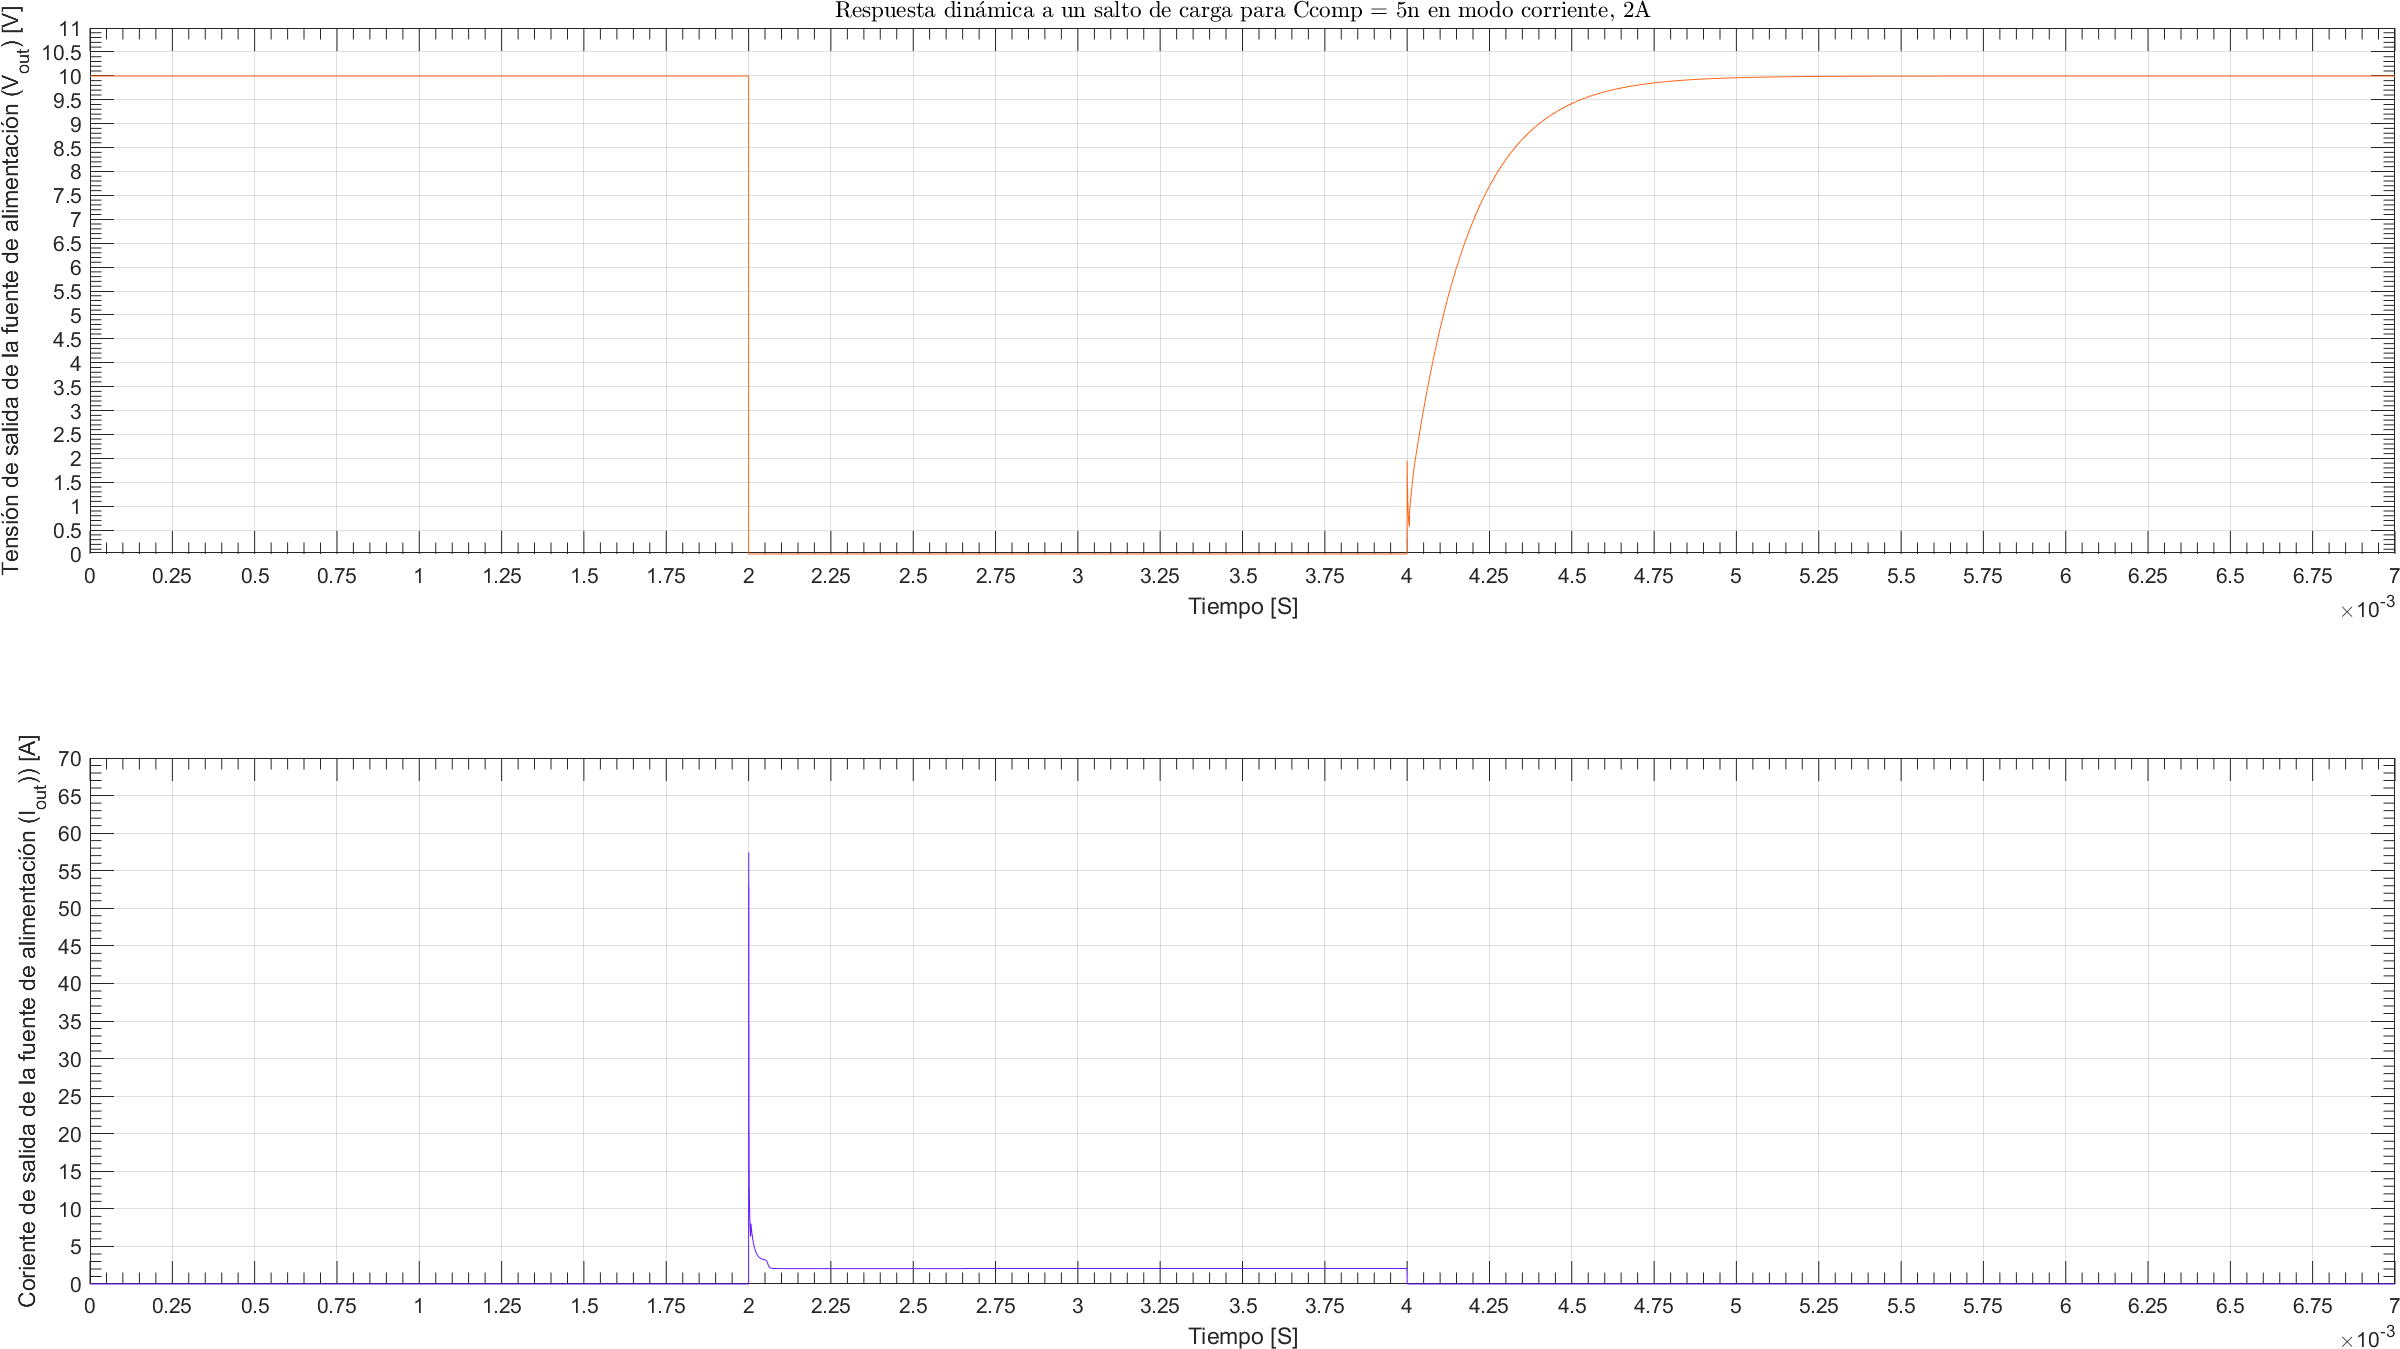
\includegraphics[width=1.1 \textwidth, angle=90]{./img/plots/dynamic/power_supply_CCOMP_5n_STEP_Modo3.png}
\caption{\label{fig:fig_power_supply_CCOMP_STEP_5n_Modo3}\footnotesize{Respuesta dinámica en modo corriente, $I_{out} = 2 \si[per-mode=symbol]{\ampere}$, para $C_{comp} = 5 \si[per-mode=symbol]{\nano\farad} $.}}
\end{center}
\end{figure}

\clearpage

\begin{figure}[H] %htb
\begin{center}
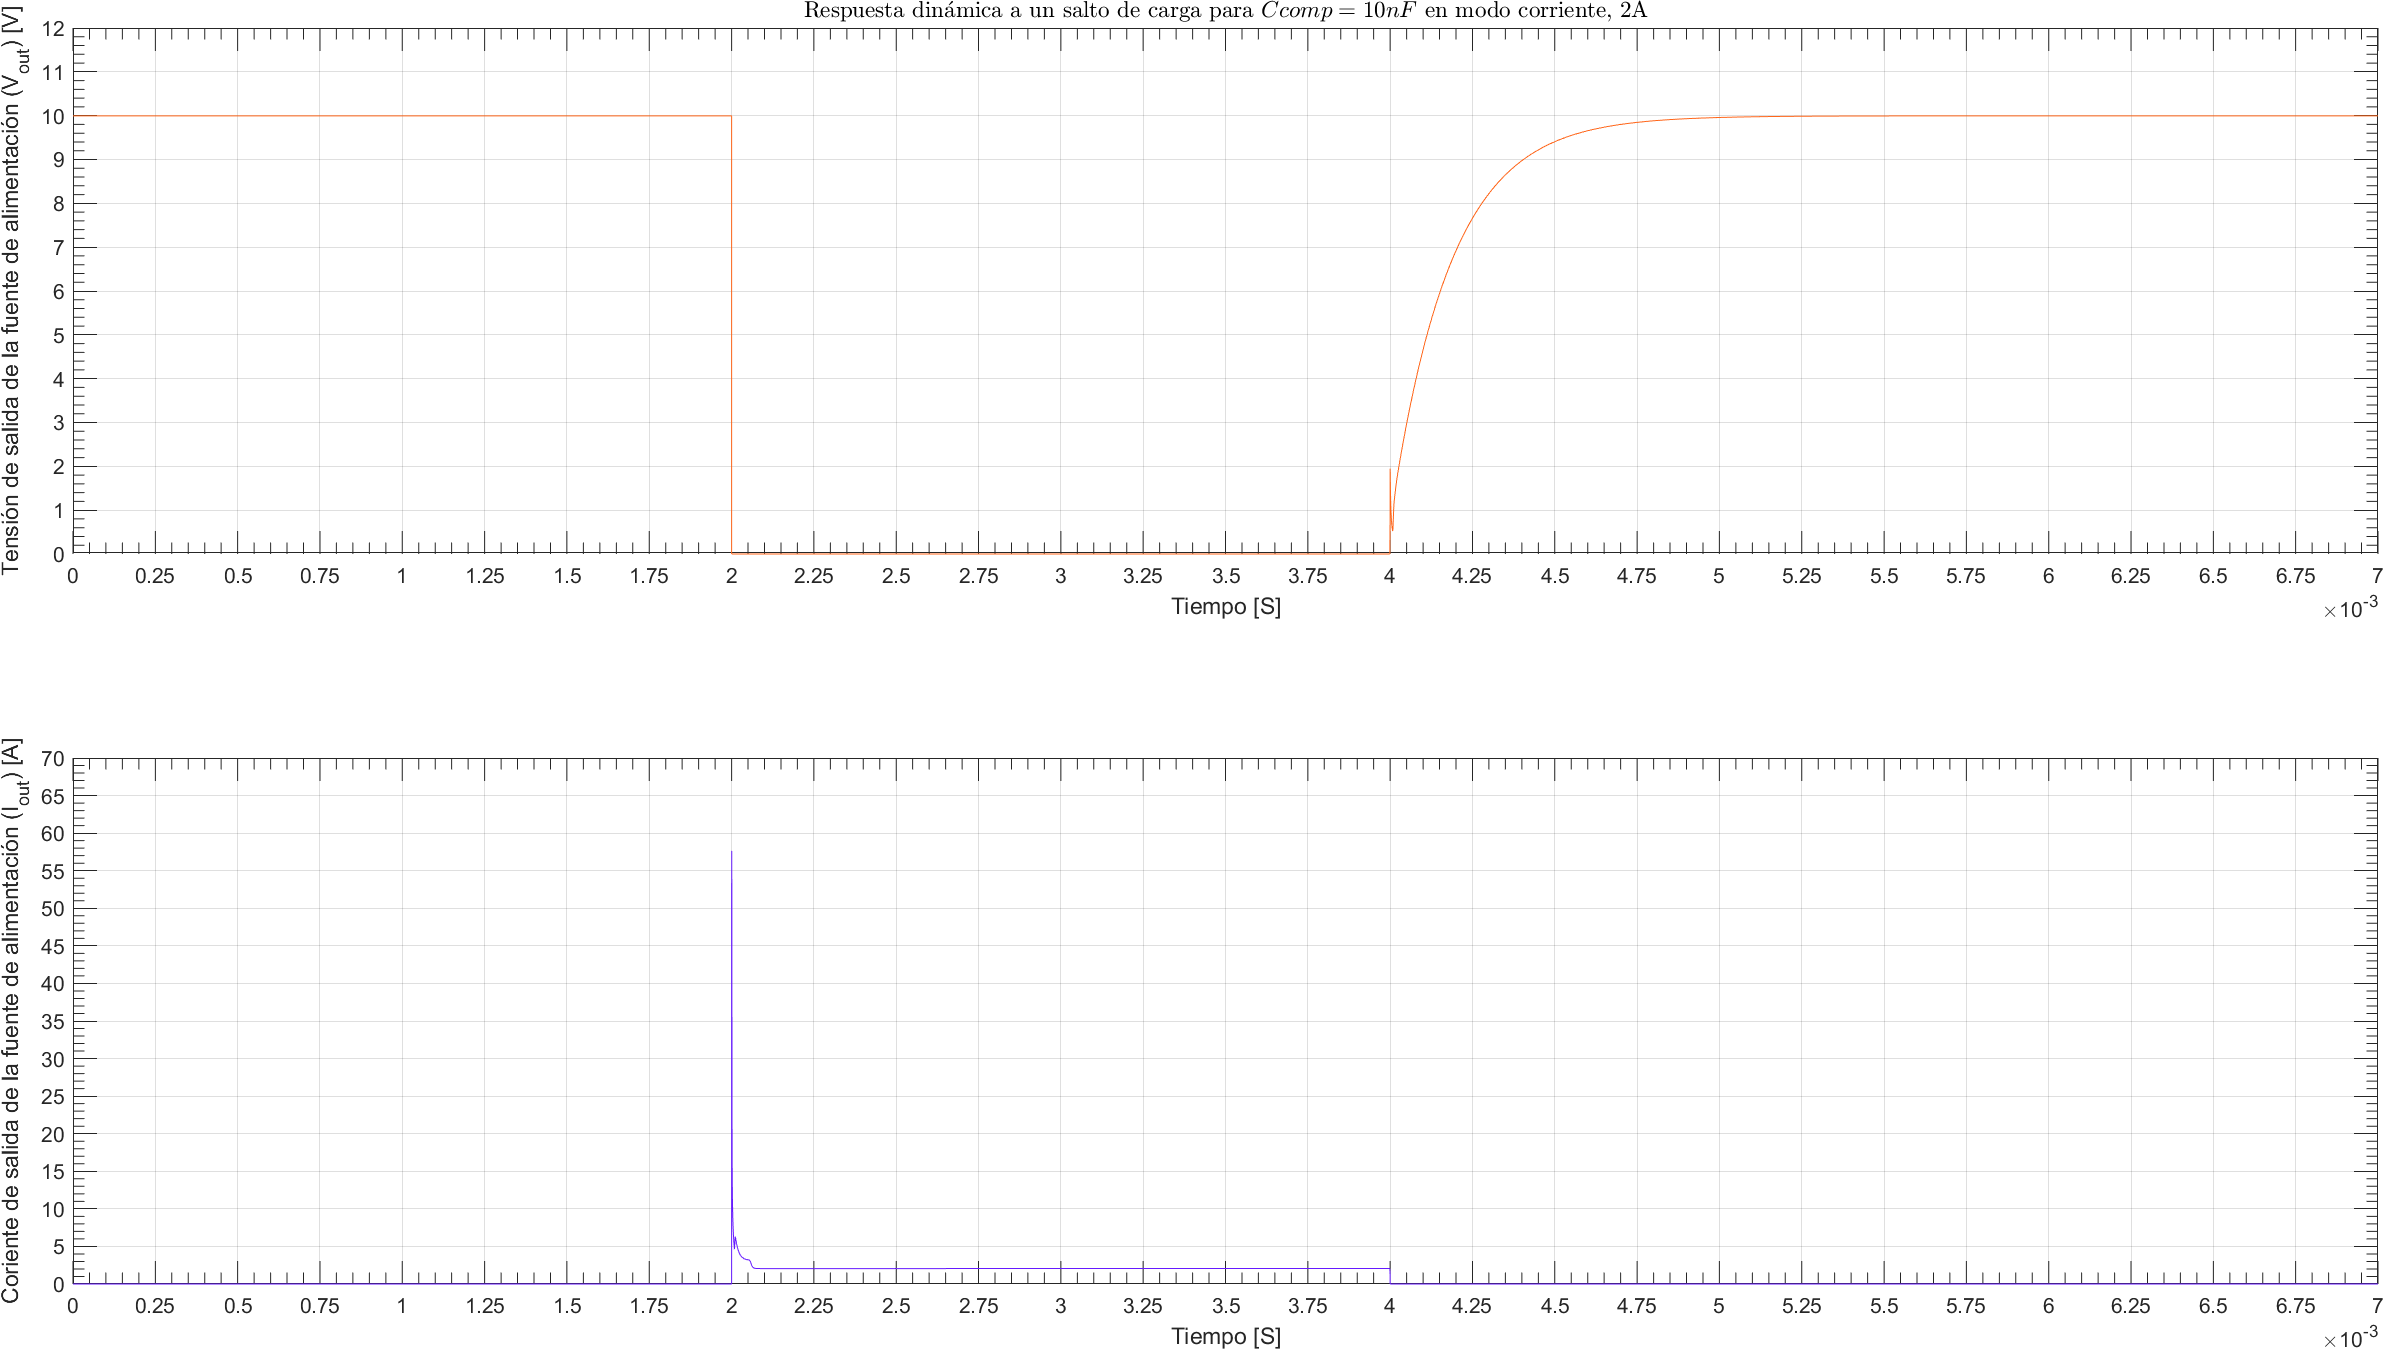
\includegraphics[width=1.1 \textwidth, angle=90]{./img/plots/dynamic/power_supply_CCOMP_10n_STEP_Modo3.png}
\caption{\label{fig:fig_power_supply_CCOMP_STEP_10n_Modo3}\footnotesize{Respuesta dinámica en modo corriente, $I_{out} = 2 \si[per-mode=symbol]{\ampere}$, para $C_{comp} = 10 \si[per-mode=symbol]{\nano\farad} $.}}
\end{center}
\end{figure}

\clearpage

\begin{figure}[H] %htb
\begin{center}
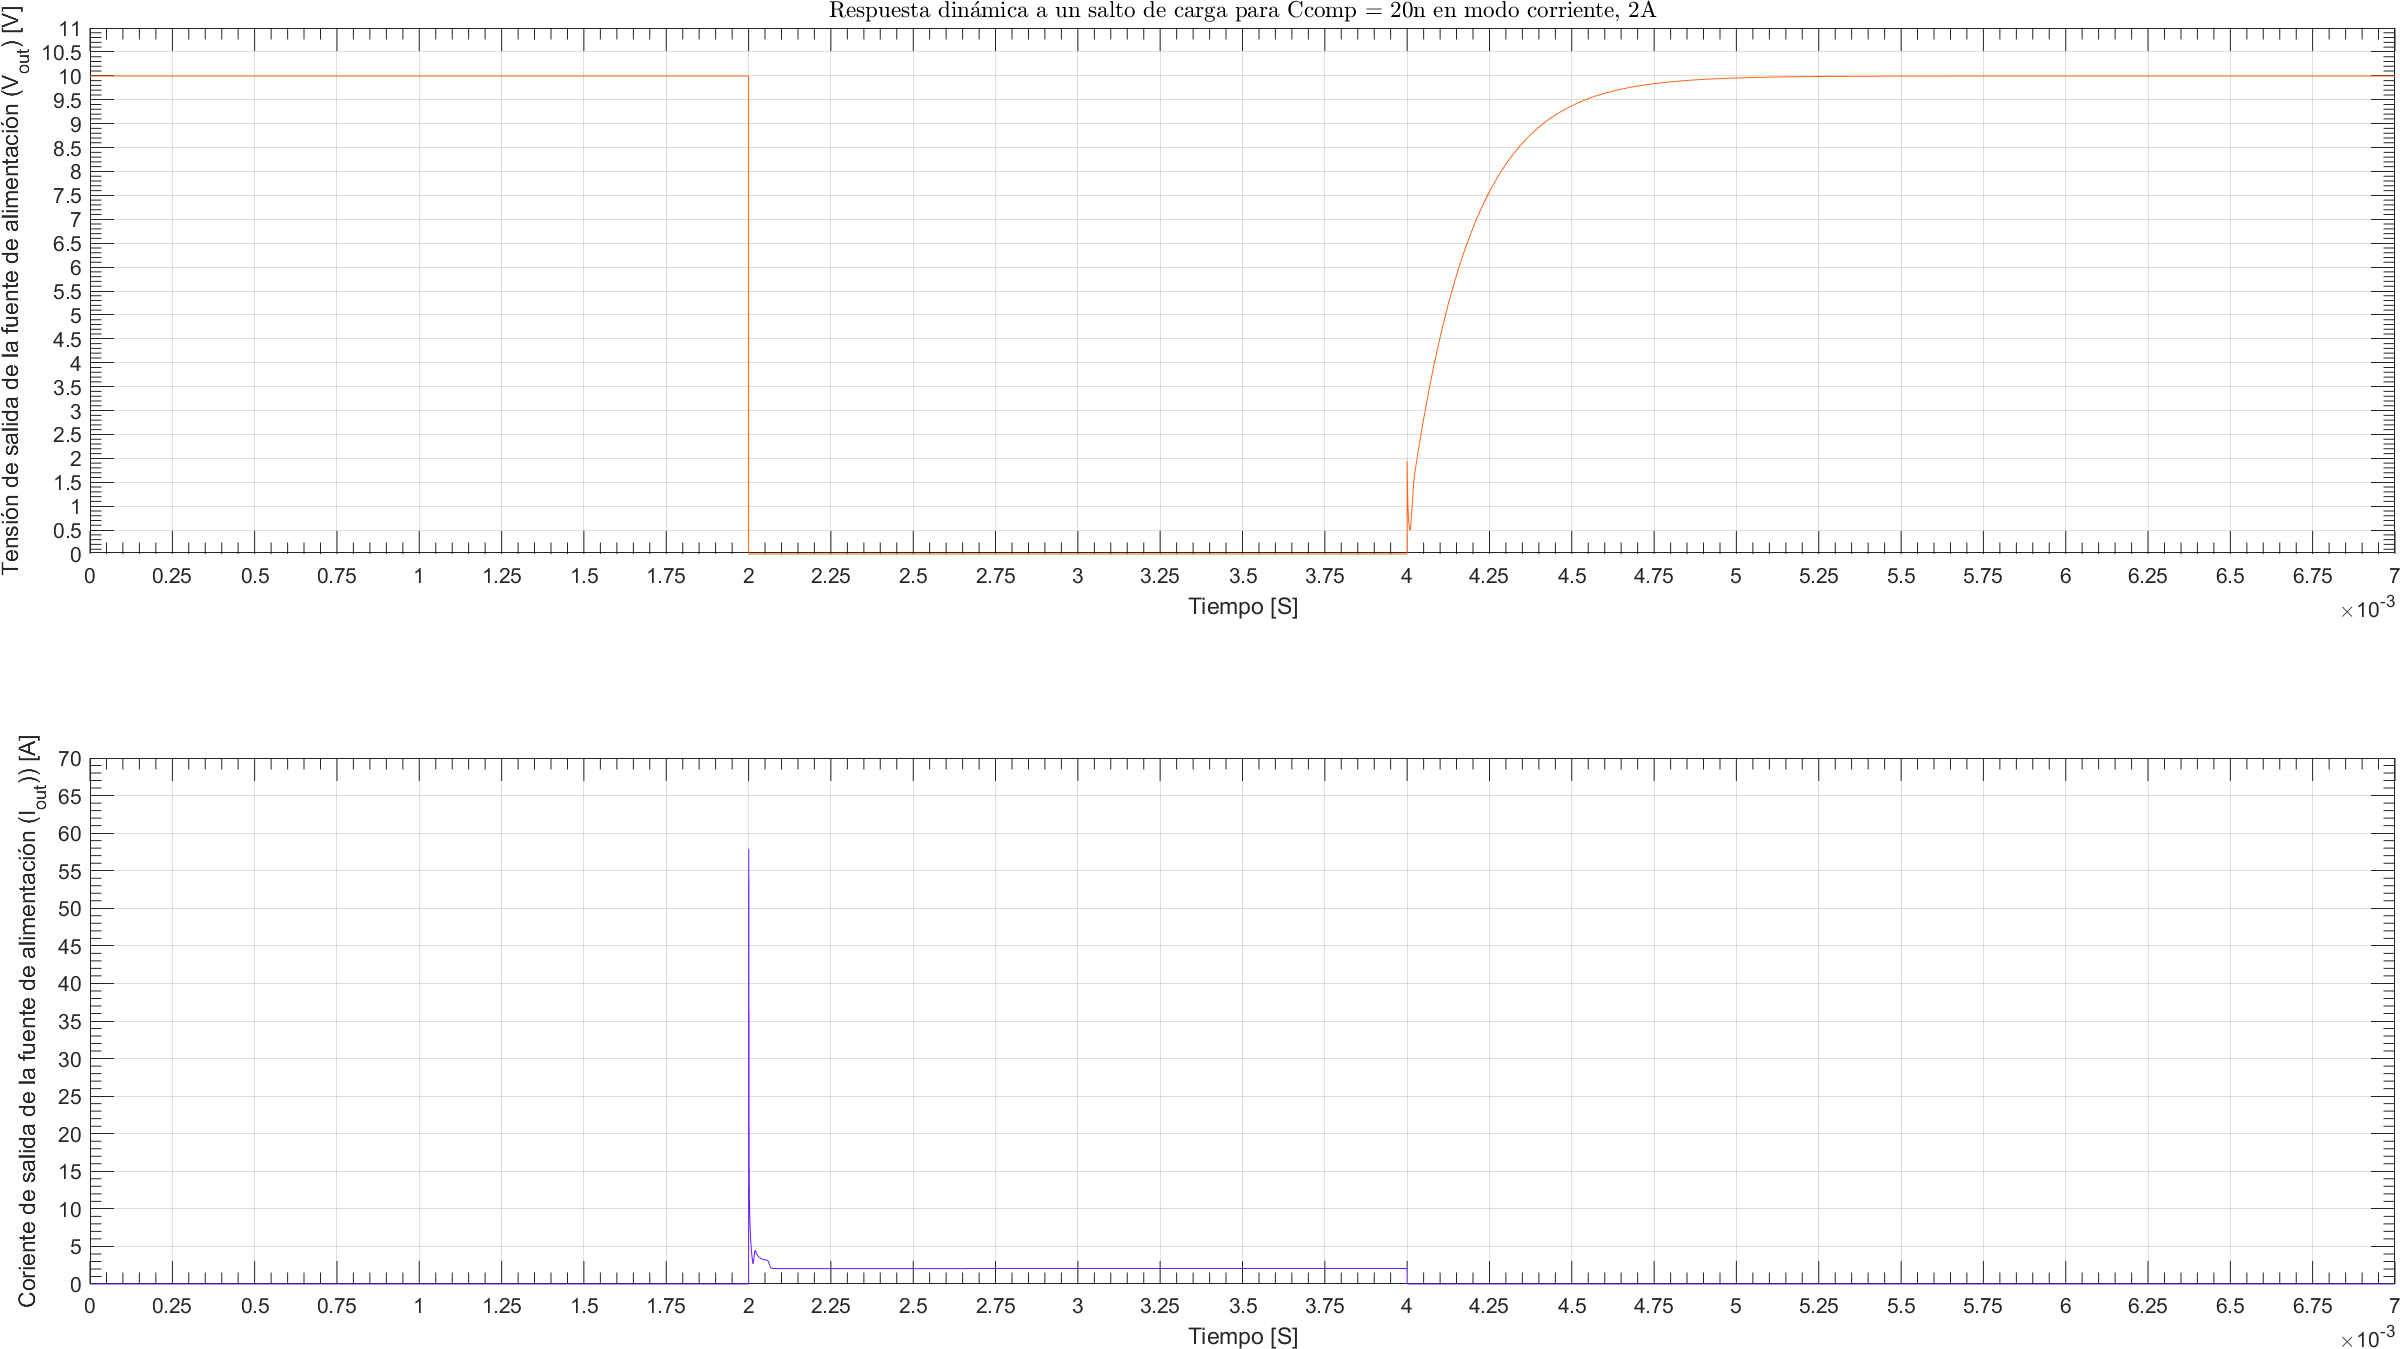
\includegraphics[width=1.1 \textwidth, angle=90]{./img/plots/dynamic/power_supply_CCOMP_20n_STEP_Modo3.png}
\caption{\label{fig:fig_power_supply_CCOMP_STEP_20n_Modo3}\footnotesize{Respuesta dinámica en modo corriente, $I_{out} = 2 \si[per-mode=symbol]{\ampere}$, para $C_{comp} = 20 \si[per-mode=symbol]{\nano\farad} $.}}
\end{center}
\end{figure}

\clearpage


\subsubsection{Análisis para $C_{comp}$ en modo corriente, $I_{out} = 200 \si[per-mode=symbol]{\milli\ampere}$, $R_{L} = 0 \si[per-mode=symbol]{\ohm}$}

Se puede ver en la figura~\figref{fig:fig_power_supply_CCOMP_LOOP_Modo4} como ya con el valor de $C_{comp} = 10 \si[per-mode=symbol]{\nano\farad}$ se logra unos márgenes de fase y ganancia positivos, pero no muy buenos, seguir aumentando el valor de $C_{comp}$, solo disminuye el ancho de banda, como se puede ver en la figura~\figref{fig:fig_power_supply_CCOMP_RF_Modo4}. A nivel de respuesta dinámica, nuevamente no se ven grandes diferencias entre los valores simulados, pero ya el tiempo de crecimiento se ve que es apreciablemte mayor que en los casos anteriores, ver figura~\figref{fig:fig_power_supply_CCOMP_STEP_5n_Modo4}, figura~\figref{fig:fig_power_supply_CCOMP_STEP_10n_Modo4} y figura~\figref{fig:fig_power_supply_CCOMP_STEP_20n_Modo4}, motivo principal para no seguir aumentando el valor de $C_{comp}$.

\vfill


% CCOMP MODO 4.

\clearpage

\begin{figure}[H] %htb
\begin{center}
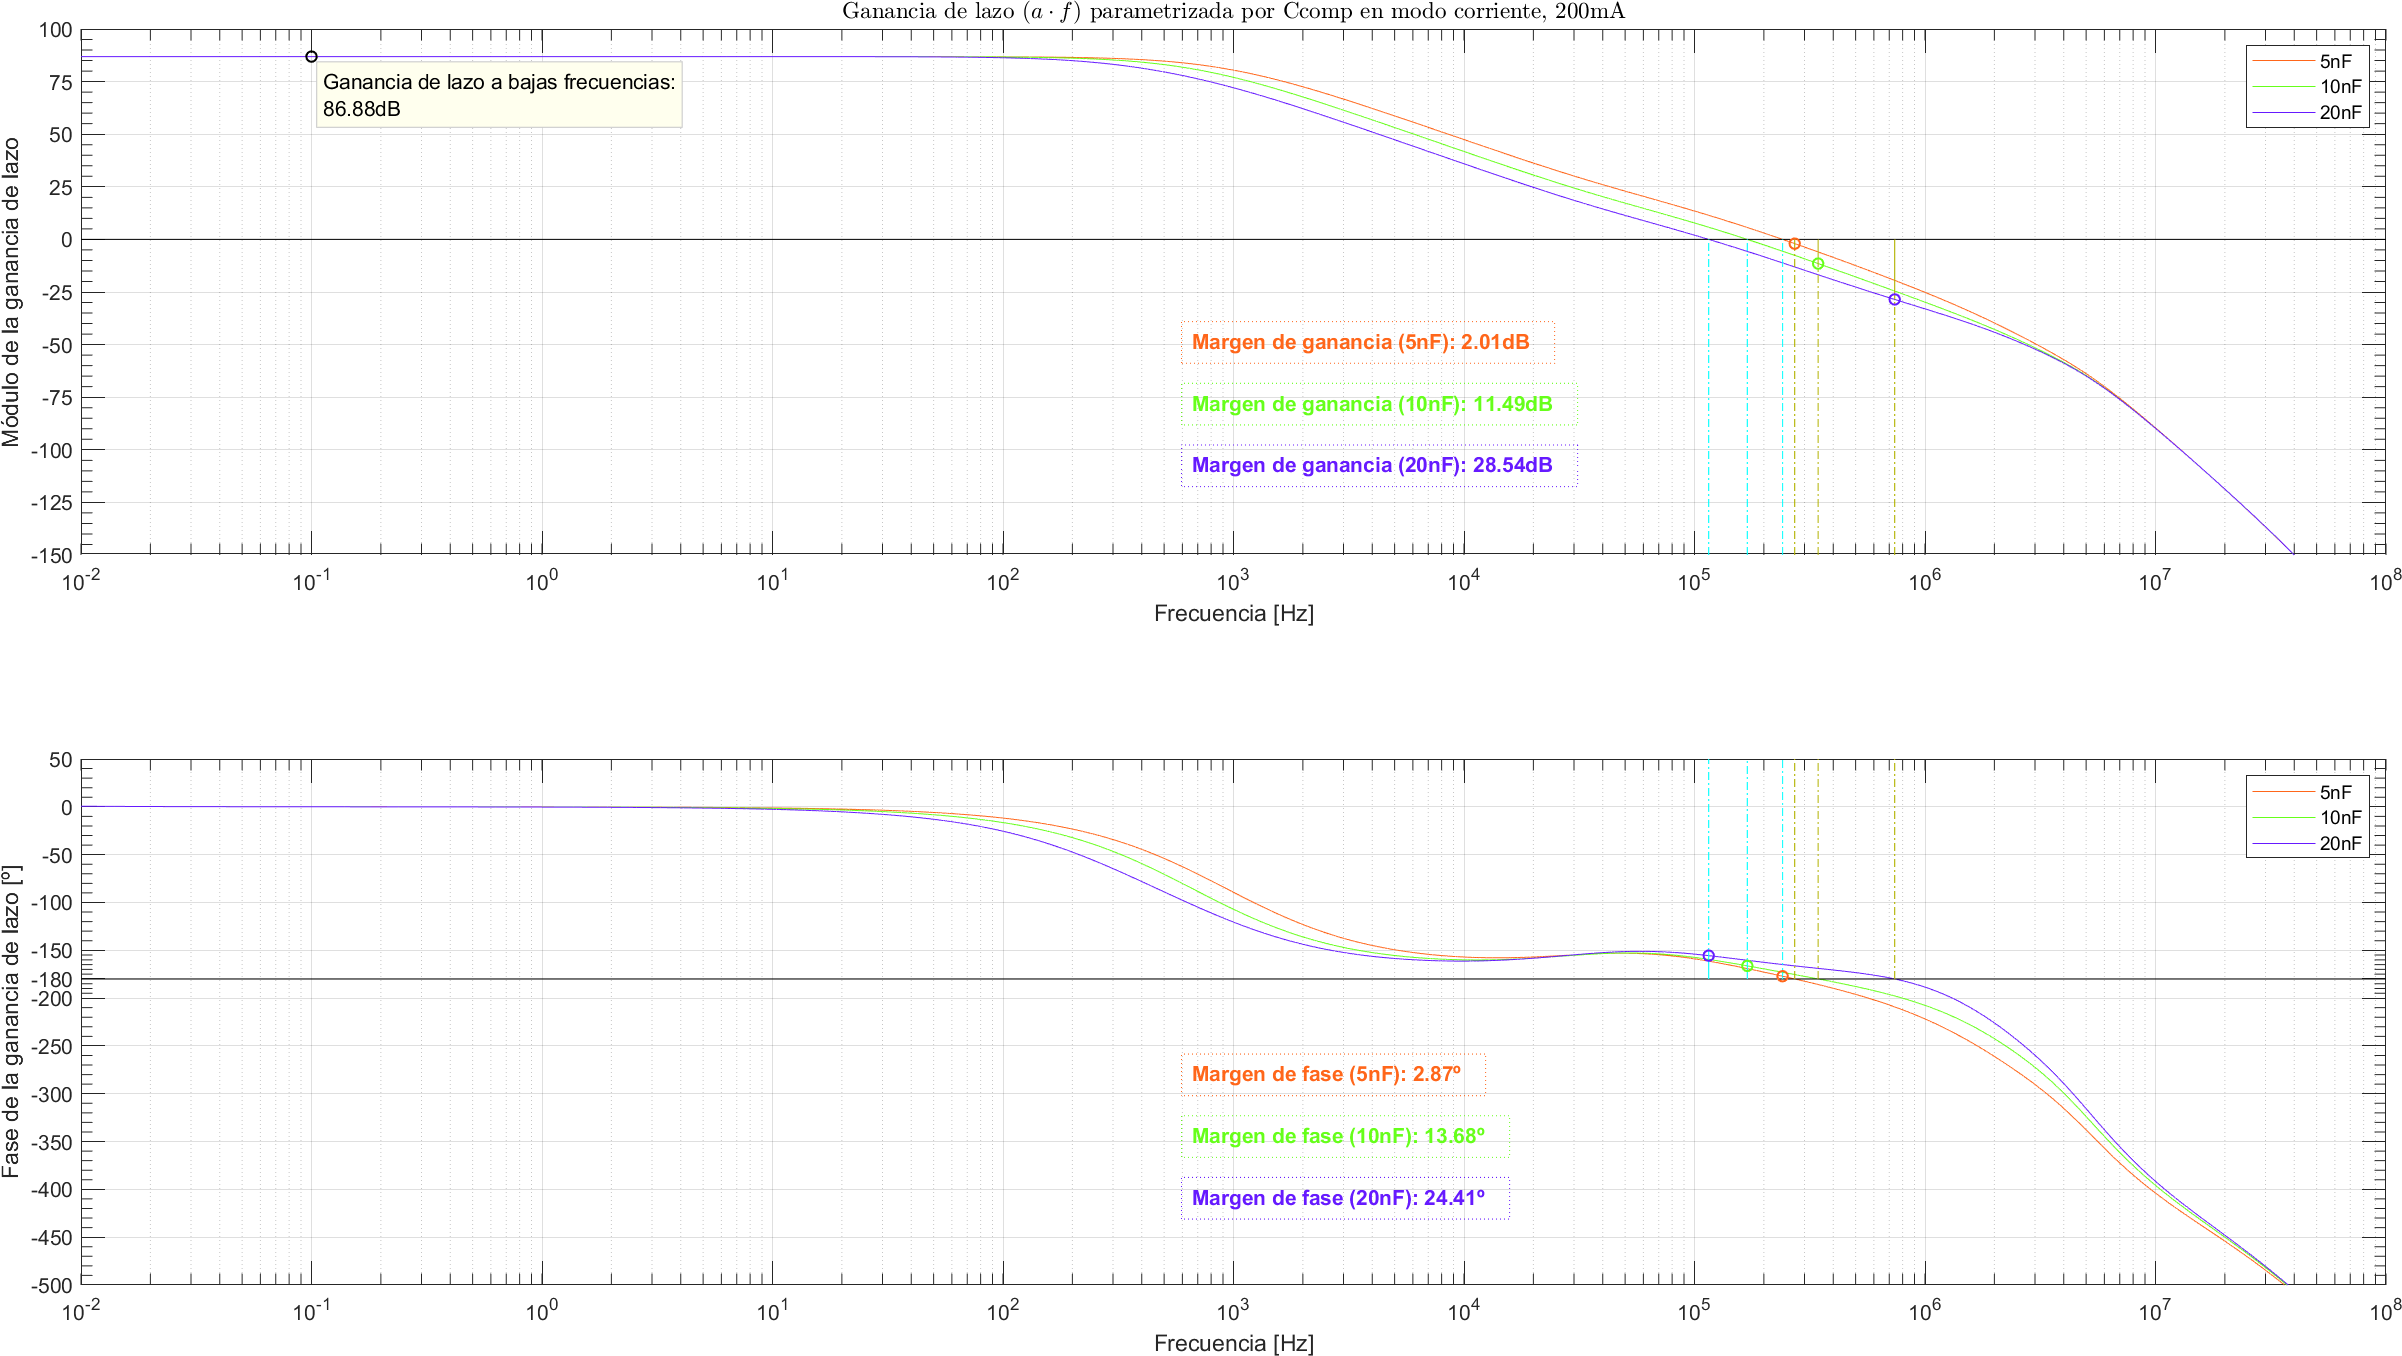
\includegraphics[width=1.1 \textwidth, angle=90]{./img/plots/loop/power_supply_CCOMP_LOOP_Modo4.png}
\caption{\label{fig:fig_power_supply_CCOMP_LOOP_Modo4}\footnotesize{Ganancia de lazo en modo corriente, $I_{out} = 200 \si[per-mode=symbol]{\milli\ampere}$, en función de la frecuencia parametrizada por $C_{comp}$.}}
\end{center}
\end{figure}


\clearpage

\begin{figure}[H] %htb
\begin{center}
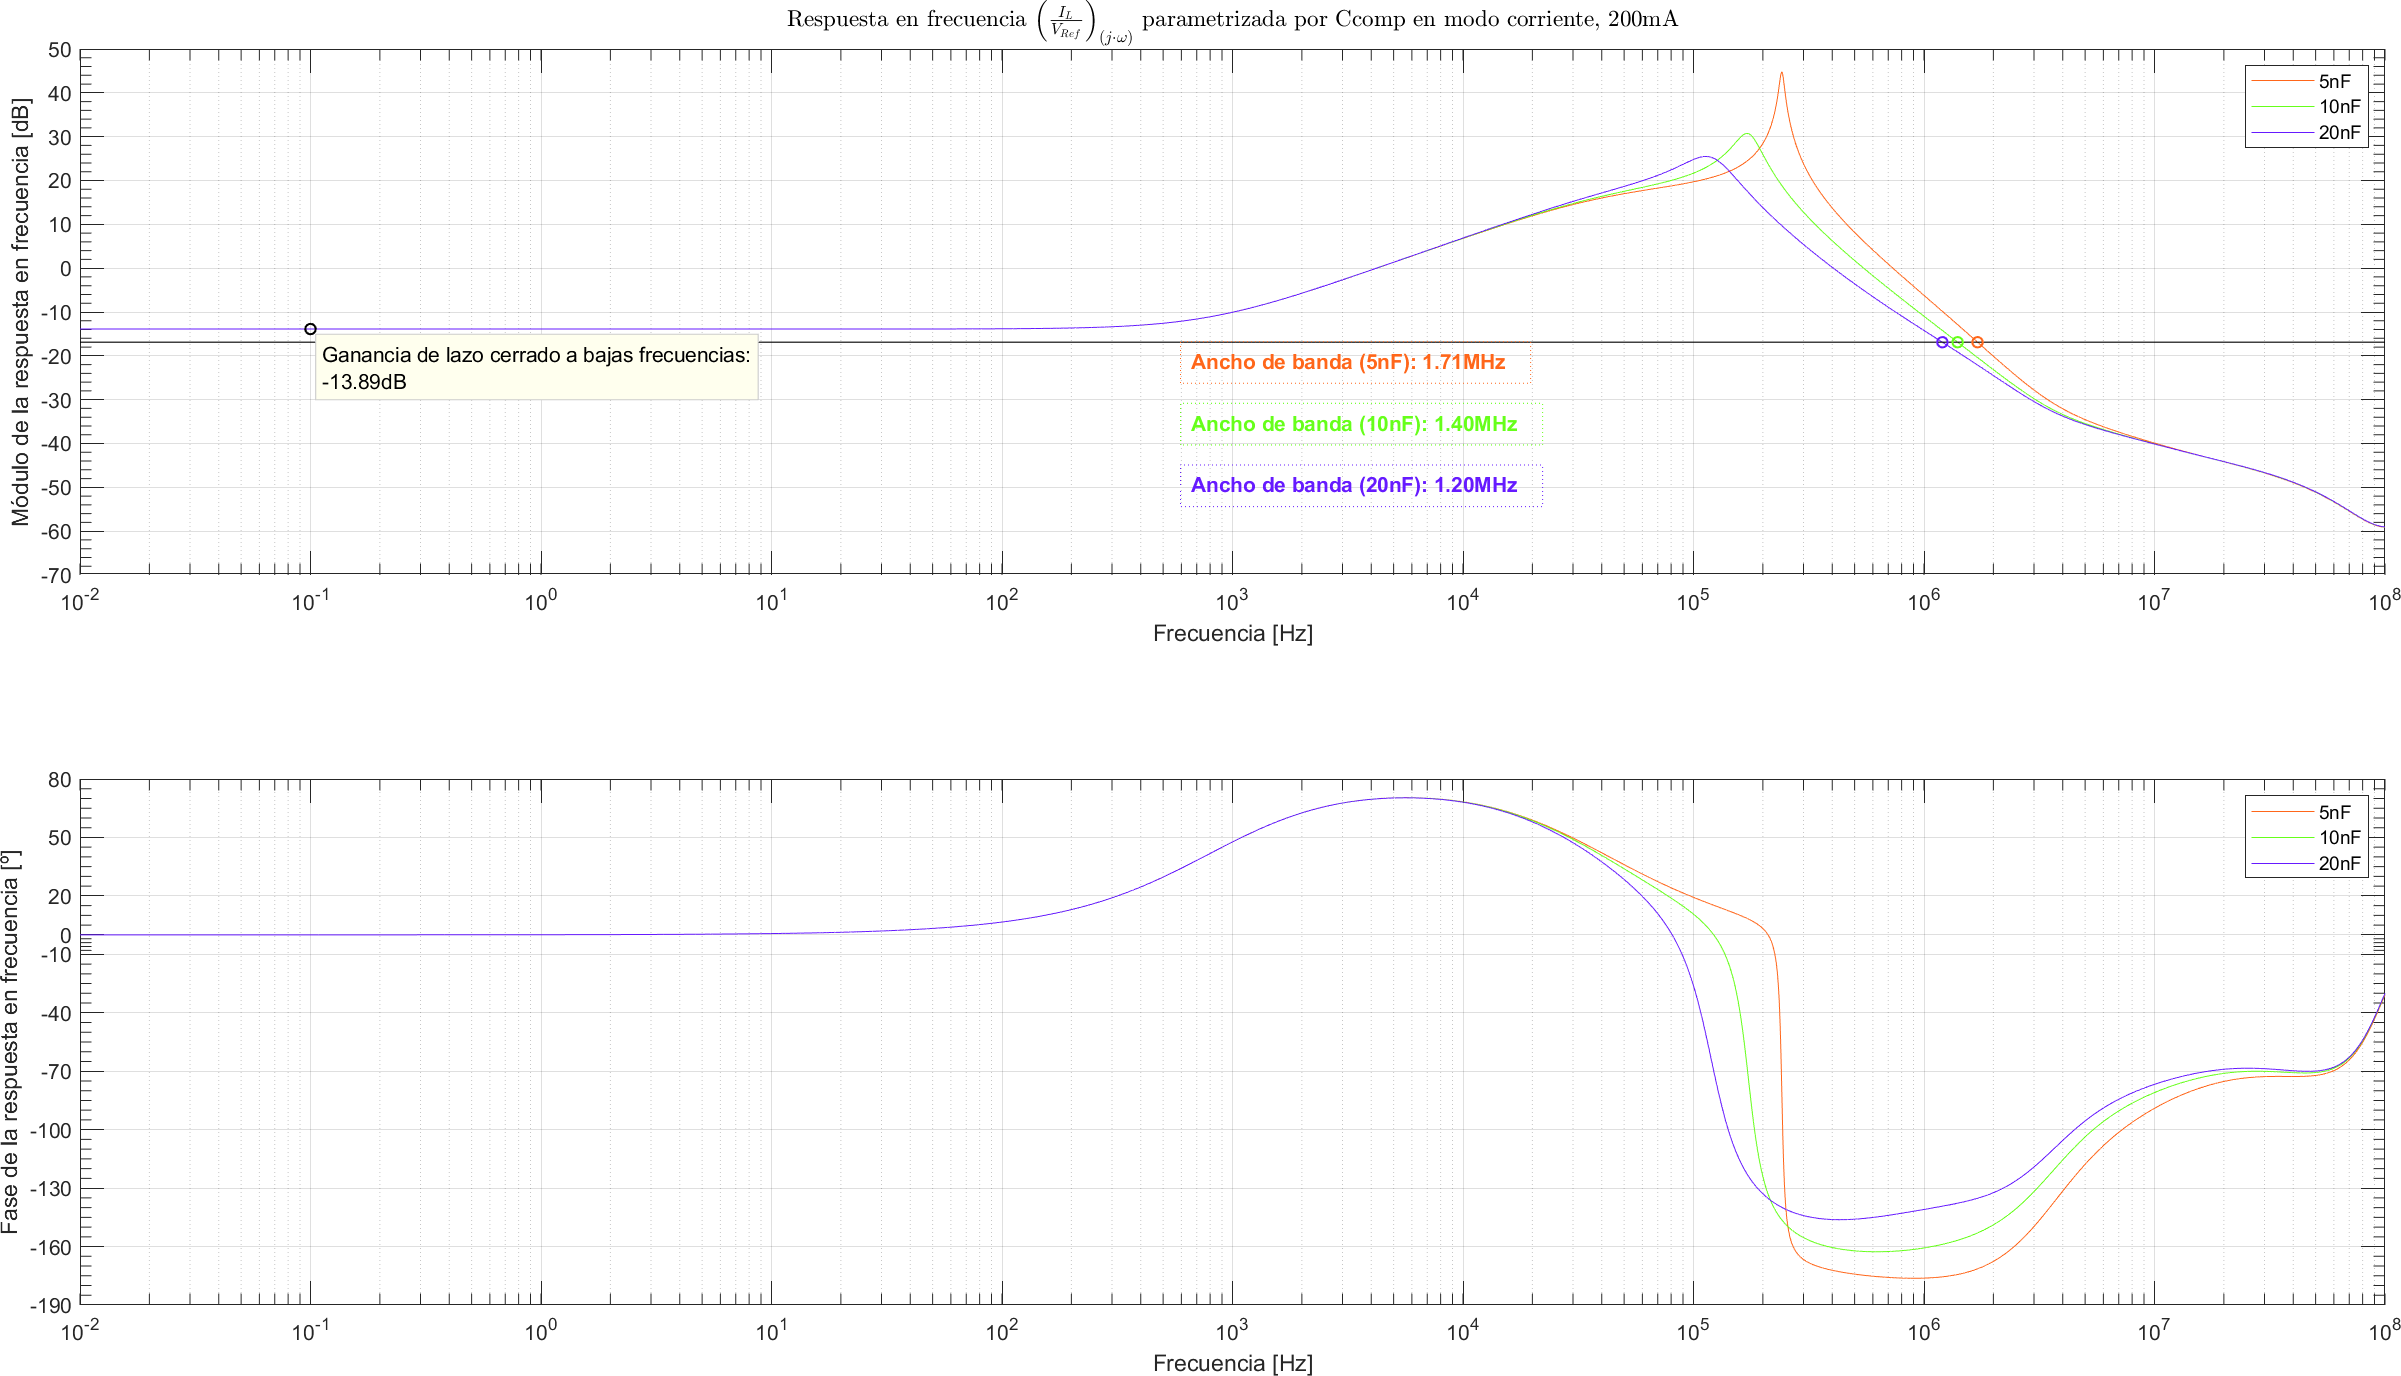
\includegraphics[width=1.1 \textwidth, angle=90]{./img/plots/rf/power_supply_CCOMP_RF_Modo4.png}
\caption{\label{fig:fig_power_supply_CCOMP_RF_Modo4}\footnotesize{Respuesta en frecuencia en modo corriente, $I_{out} = 200 \si[per-mode=symbol]{\milli\ampere}$, en función de la frecuencia parametrizada por $C_{comp}$.}}
\end{center}
\end{figure}

\clearpage

\begin{figure}[H] %htb
\begin{center}
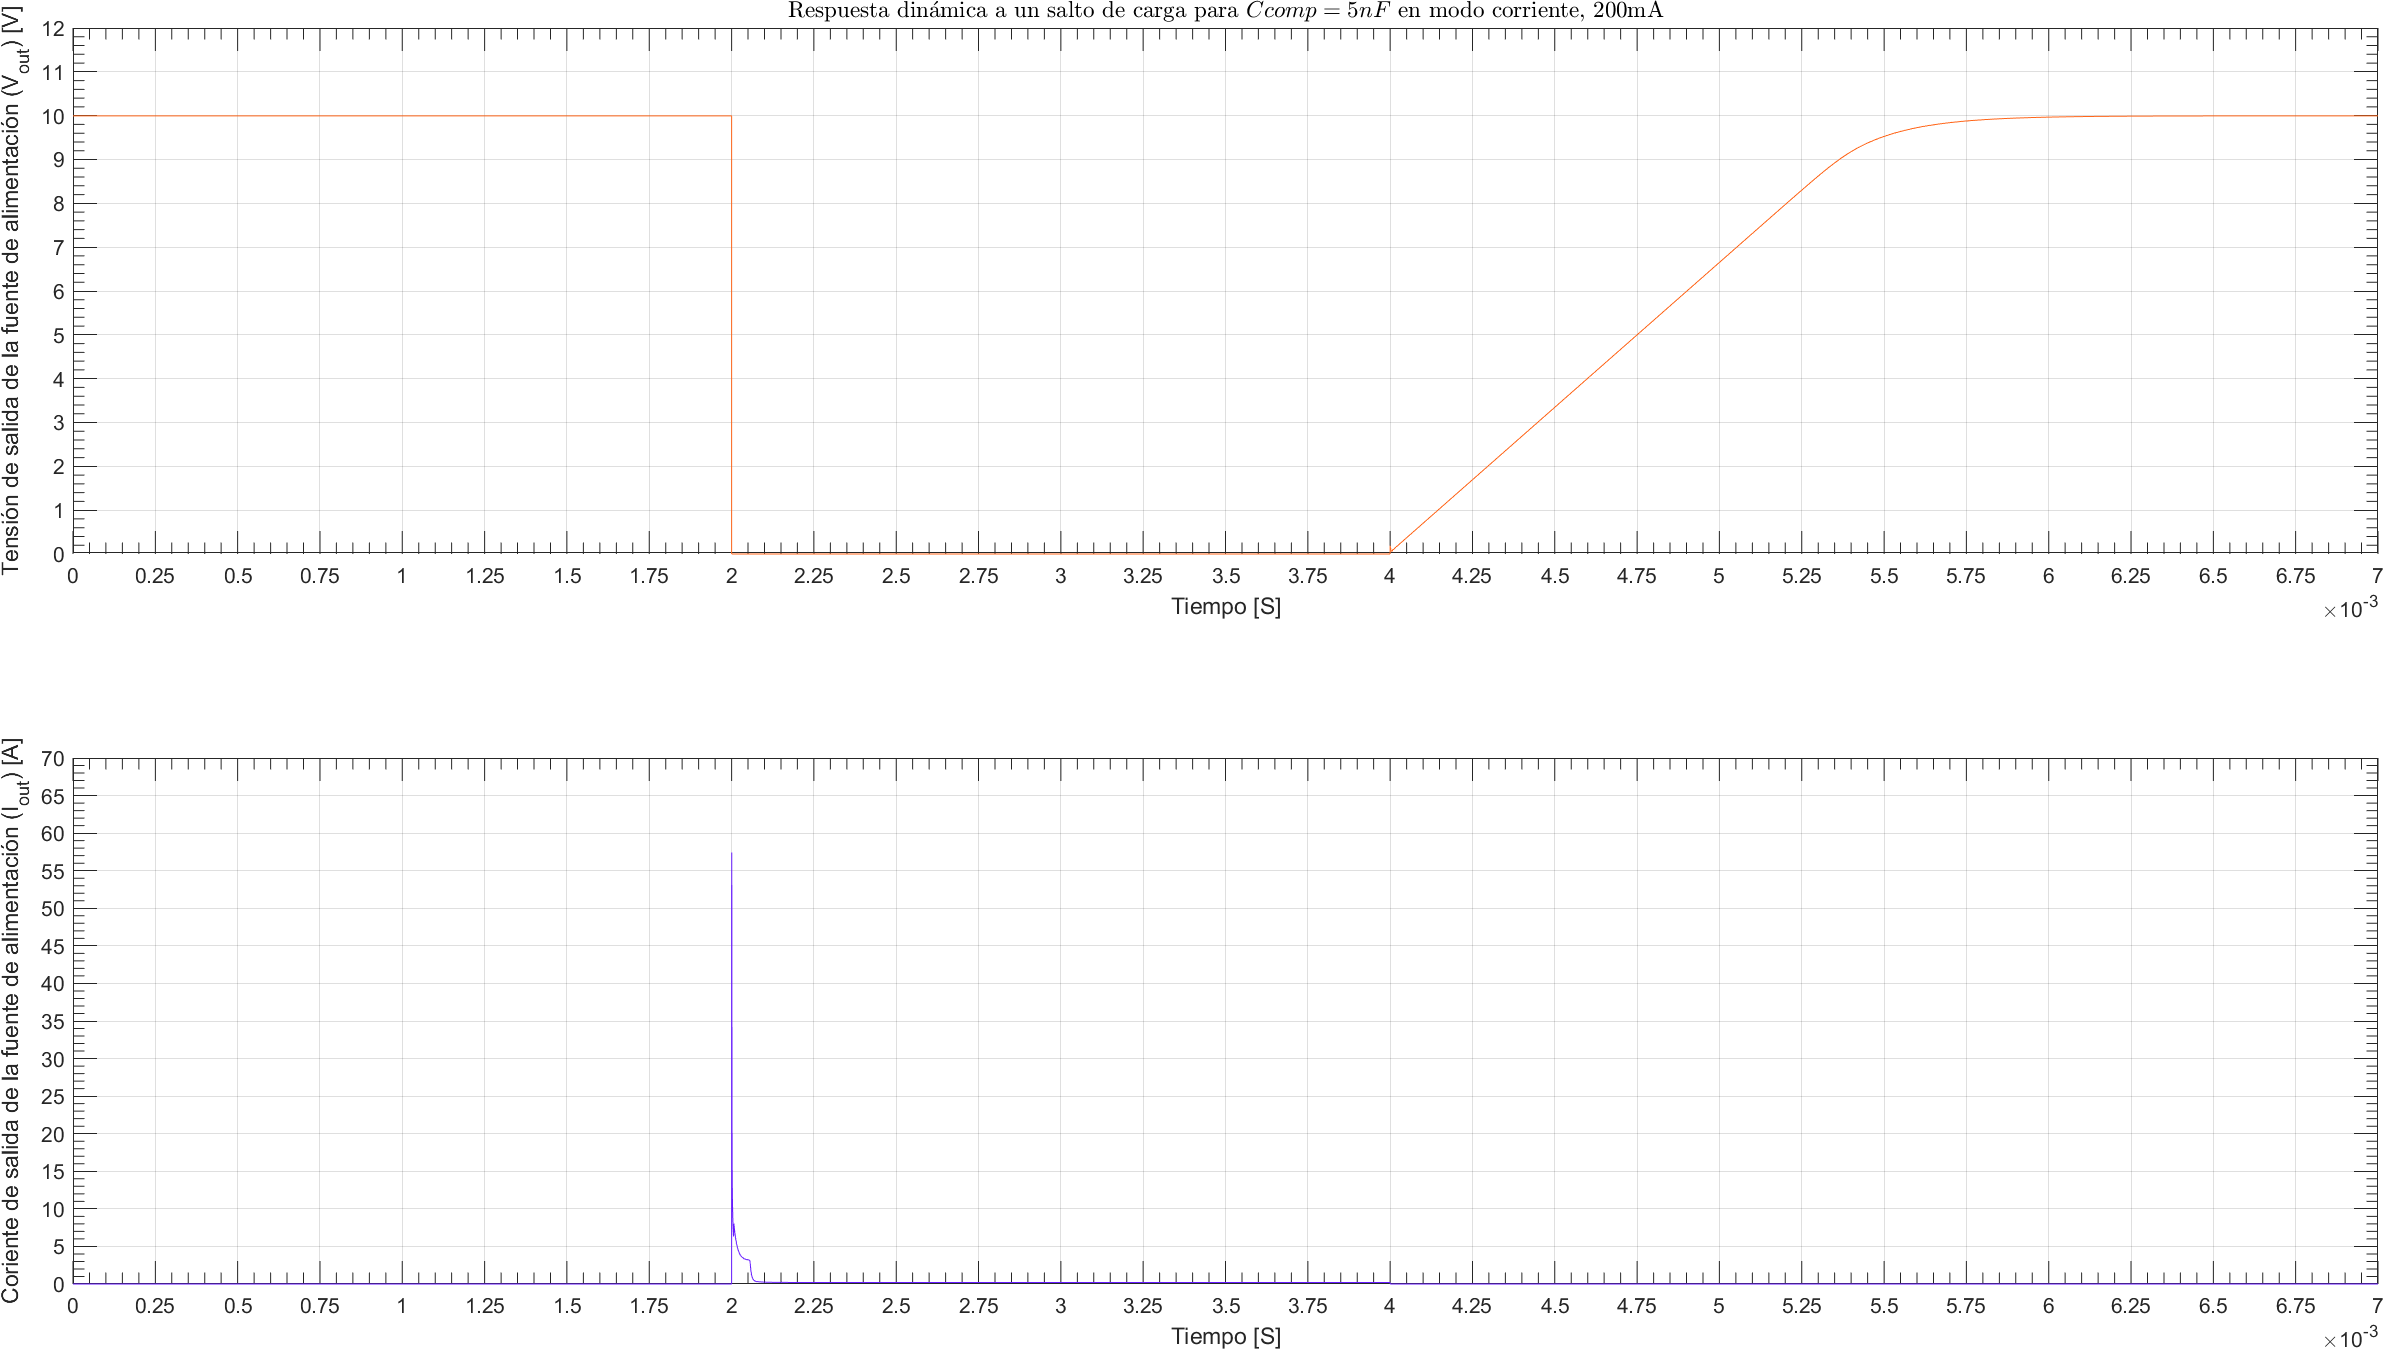
\includegraphics[width=1.1 \textwidth, angle=90]{./img/plots/dynamic/power_supply_CCOMP_5n_STEP_Modo4.png}
\caption{\label{fig:fig_power_supply_CCOMP_STEP_5n_Modo4}\footnotesize{Respuesta dinámica en modo corriente, $I_{out} = 200 \si[per-mode=symbol]{\milli\ampere}$, para $C_{comp} = 5 \si[per-mode=symbol]{\nano\farad} $.}}
\end{center}
\end{figure}

\clearpage

\begin{figure}[H] %htb
\begin{center}
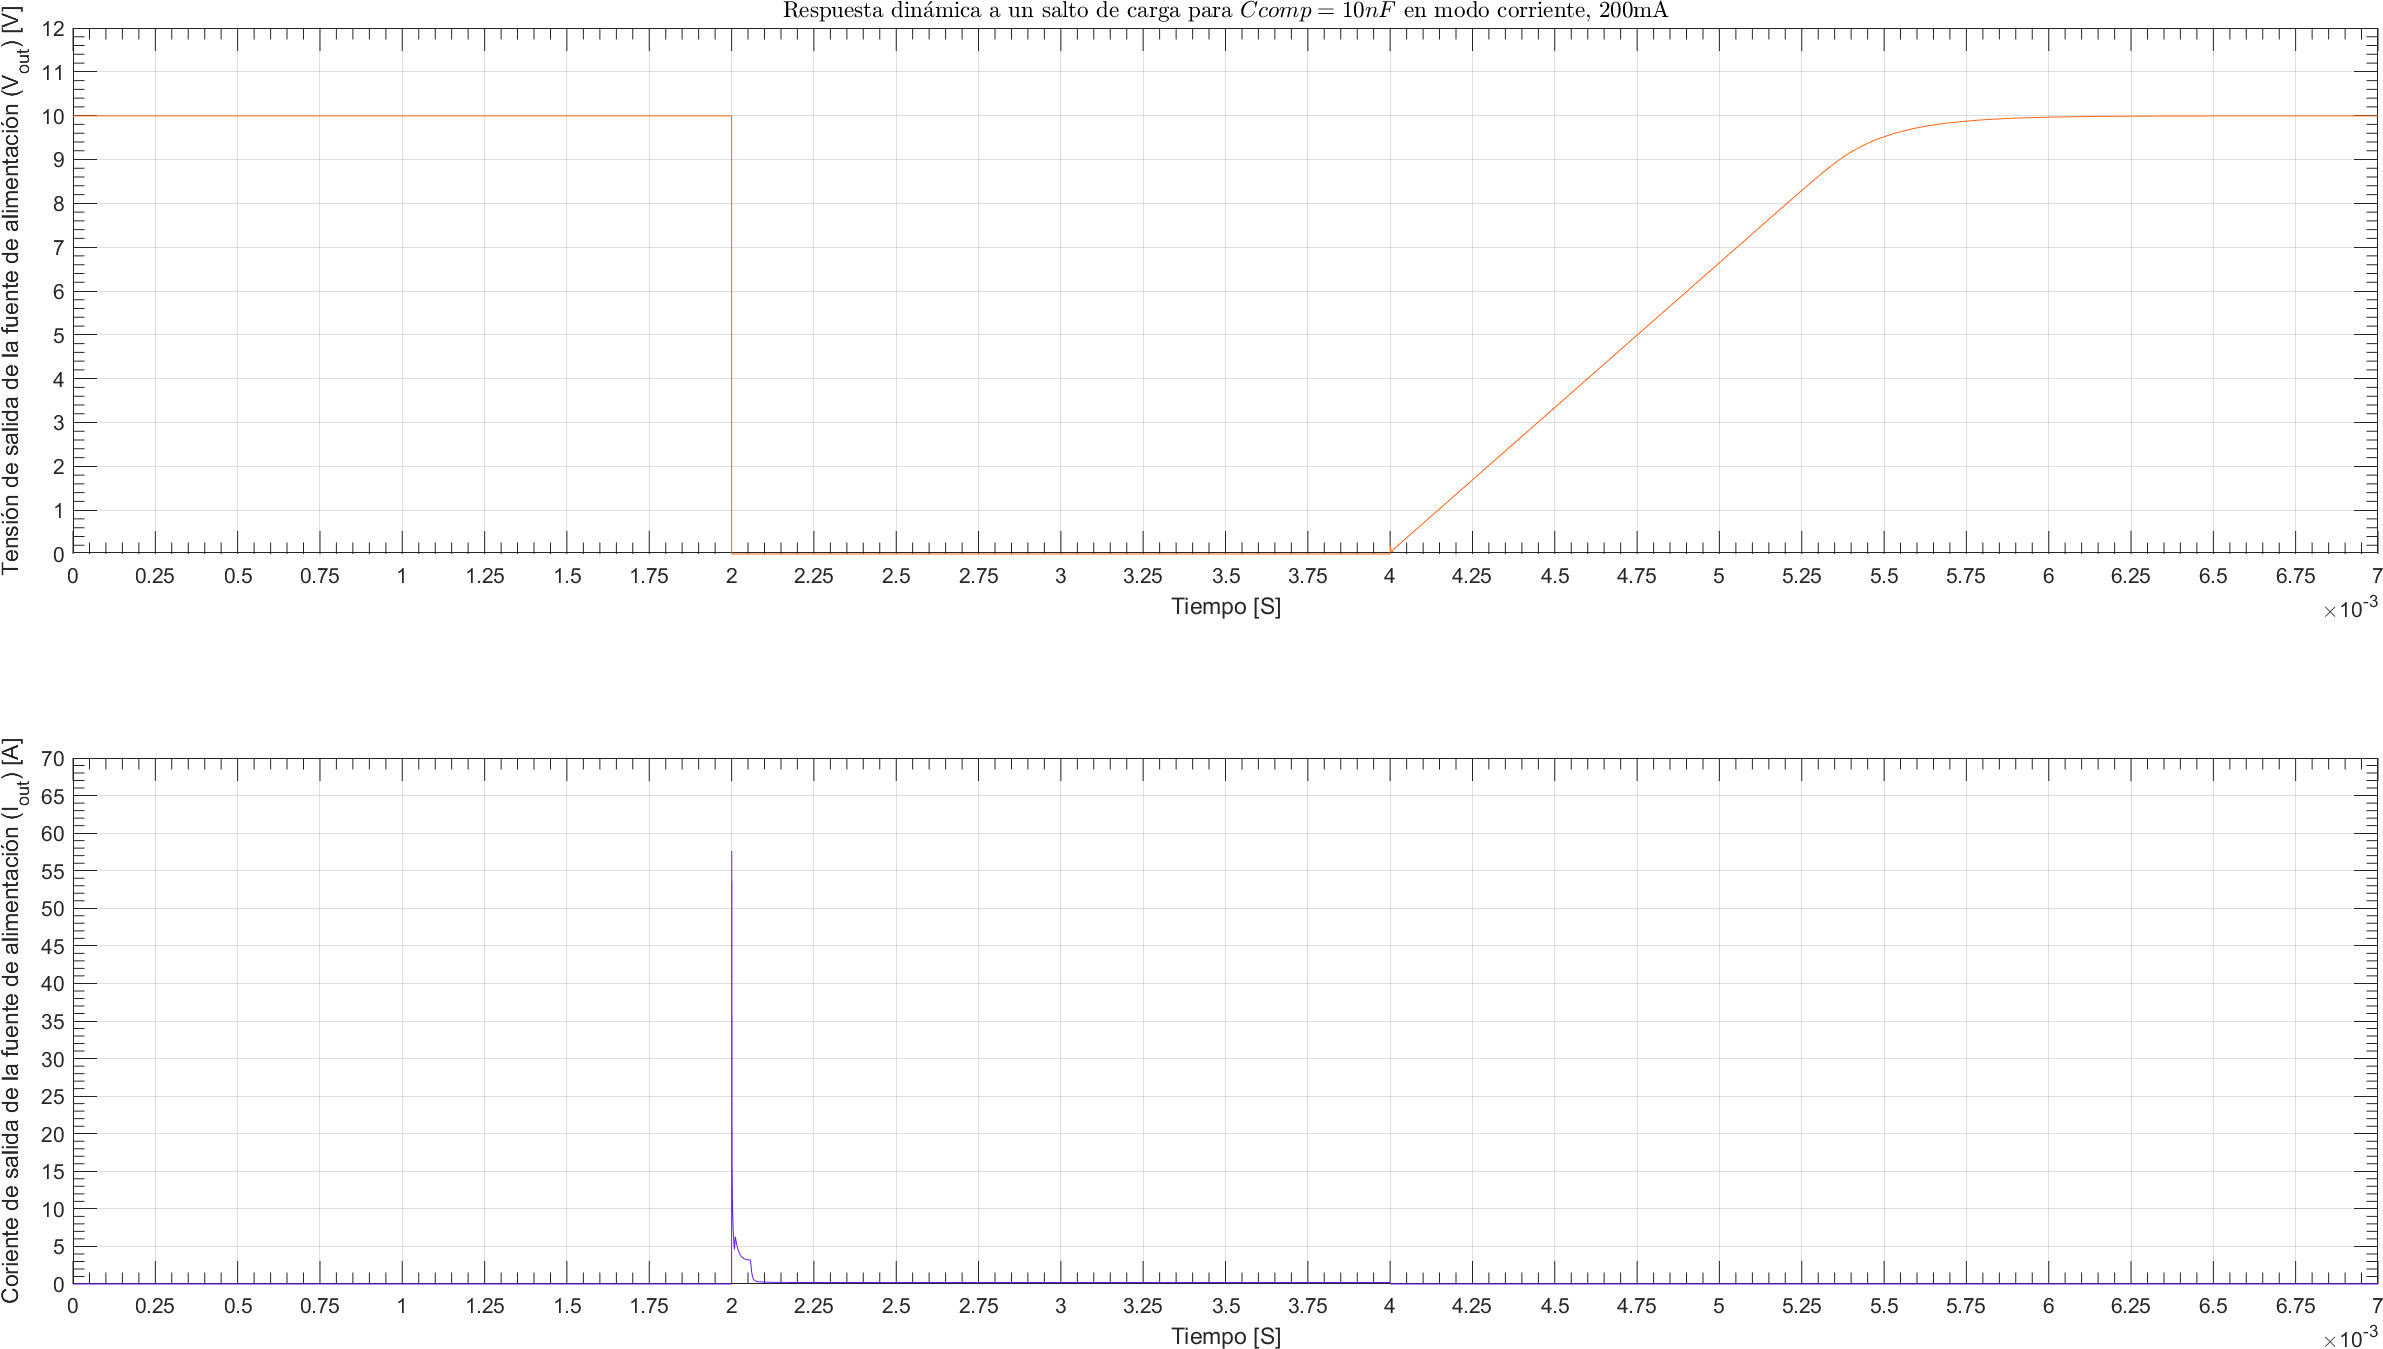
\includegraphics[width=1.1 \textwidth, angle=90]{./img/plots/dynamic/power_supply_CCOMP_10n_STEP_Modo4.png}
\caption{\label{fig:fig_power_supply_CCOMP_STEP_10n_Modo4}\footnotesize{Respuesta dinámica en modo corriente, $I_{out} = 200 \si[per-mode=symbol]{\milli\ampere}$, para $C_{comp} = 10 \si[per-mode=symbol]{\nano\farad} $.}}
\end{center}
\end{figure}

\clearpage

\begin{figure}[H] %htb
\begin{center}
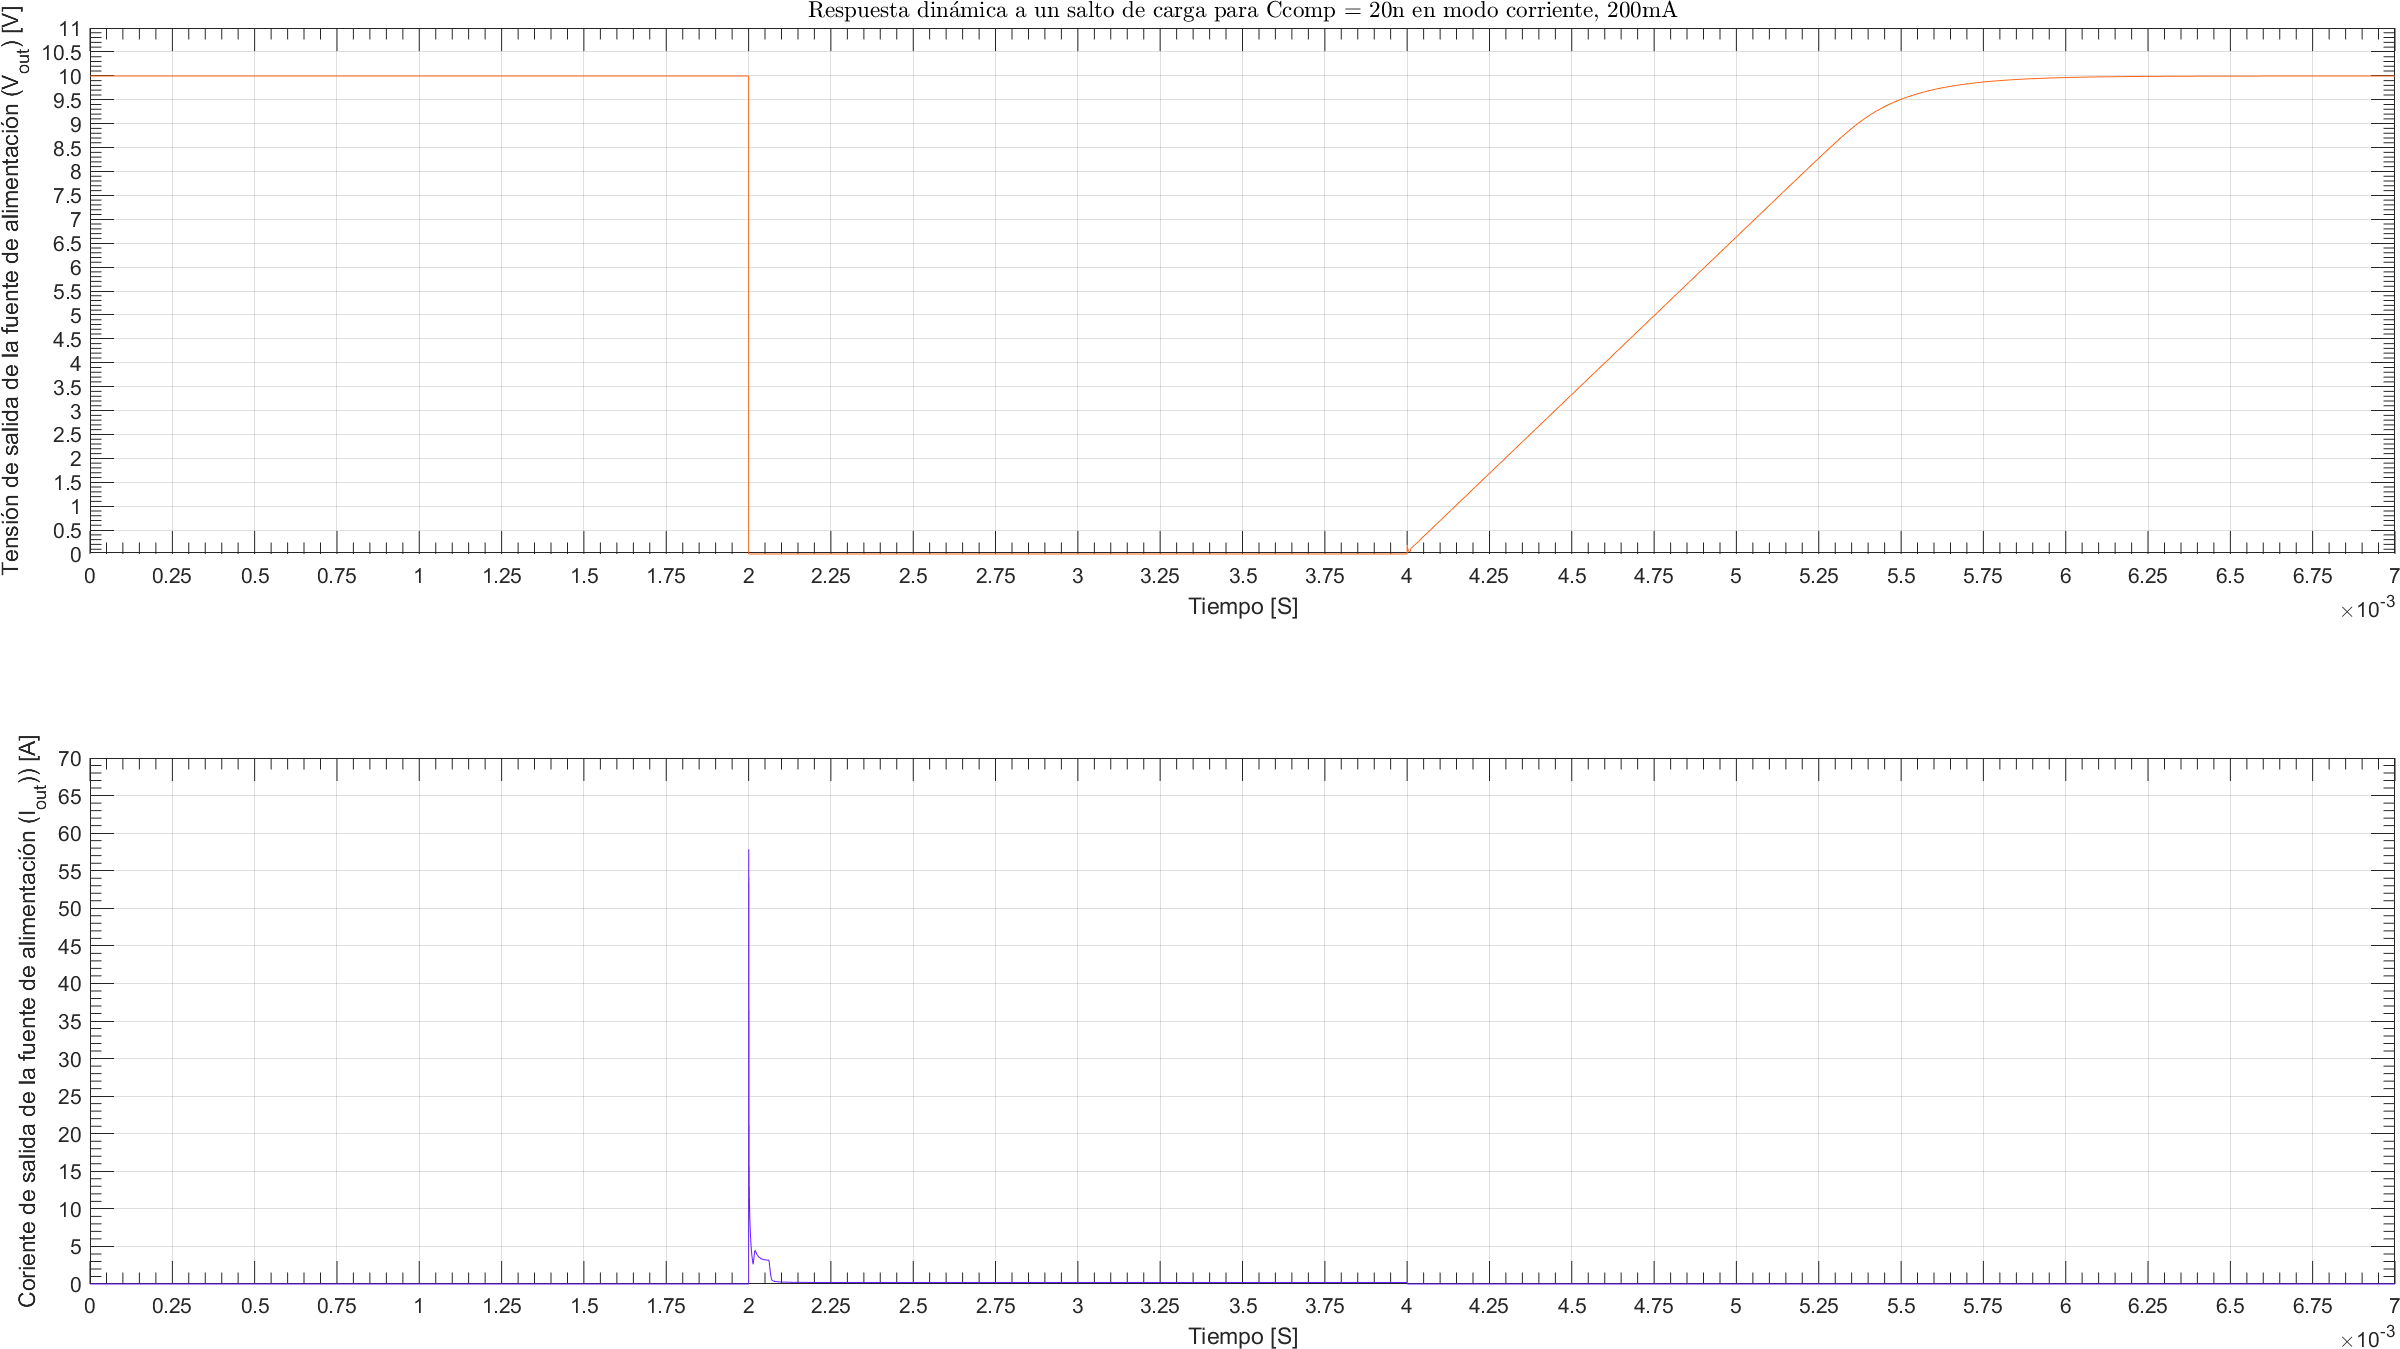
\includegraphics[width=1.1 \textwidth, angle=90]{./img/plots/dynamic/power_supply_CCOMP_20n_STEP_Modo4.png}
\caption{\label{fig:fig_power_supply_CCOMP_STEP_20n_Modo4}\footnotesize{Respuesta dinámica en modo corriente, $I_{out} = 200 \si[per-mode=symbol]{\milli\ampere}$, para $C_{comp} = 20 \si[per-mode=symbol]{\nano\farad} $.}}
\end{center}
\end{figure}

\clearpage




